%%%%%%%% ICML 2021 EXAMPLE LATEX SUBMISSION FILE %%%%%%%%%%%%%%%%%

\documentclass{article}

% Recommended, but optional, packages for figures and better typesetting:
\usepackage{microtype}
\usepackage{graphicx}
%\usepackage{subfigure}
\usepackage{booktabs} % for professional tables
\usepackage{amsfonts}
\usepackage{multirow}
\usepackage{amsmath}
\usepackage{caption}
\usepackage{subcaption}
\usepackage{natbib}
%\usepackage[T1]{fontenc}

% hyperref makes hyperlinks in the resulting PDF.
% If your build breaks (sometimes temporarily if a hyperlink spans a page)
% please comment out the following usepackage line and replace
% \usepackage{icml2021} with \usepackage[nohyperref]{icml2021} above.
\usepackage{hyperref}

% Attempt to make hyperref and algorithmic work together better:
\newcommand{\theHalgorithm}{\arabic{algorithm}}

% Use the following line for the initial blind version submitted for review:
\usepackage{icml2021}

% If accepted, instead use the following line for the camera-ready submission:
%\usepackage[accepted]{icml2021}

% The \icmltitle you define below is probably too long as a header.
% Therefore, a short form for the running title is supplied here:
\icmltitlerunning{TDHNN: Time-Dependent Hamiltonian Neural Networks}

\bibliographystyle{icml2021}
\begin{document}

\twocolumn[
\icmltitle{Port-Hamiltonian Neural Networks for Learning Explicit Time-Dependent Dynamical Systems}

% It is OKAY to include author information, even for blind
% submissions: the style file will automatically remove it for you
% unless you've provided the [accepted] option to the icml2021
% package.

% List of affiliations: The first argument should be a (short)
% identifier you will use later to specify author affiliations
% Academic affiliations should list Department, University, City, Region, Country
% Industry affiliations should list Company, City, Region, Country

% You can specify symbols, otherwise they are numbered in order.
% Ideally, you should not use this facility. Affiliations will be numbered
% in order of appearance and this is the preferred way.
%\icmlsetsymbol{equal}{*}

\begin{icmlauthorlist}
\icmlauthor{Shaan Desai}{to,goo}
\icmlauthor{Marios Mattheakis}{goo}
\icmlauthor{David Sondak}{goo}
\icmlauthor{Pavlos Protopapas}{goo}
\icmlauthor{Stephen J. Roberts}{to}
\end{icmlauthorlist}

\icmlaffiliation{to}{Machine Learning Research Group , University of Oxford }
\icmlaffiliation{goo}{School of Engineering and Applied Science, Harvard University}

\icmlcorrespondingauthor{Shaan Desai}{shaan@robots.ox.ac.uk}

% You may provide any keywords that you
% find helpful for describing your paper; these are used to populate
% the "keywords" metadata in the PDF but will not be shown in the document
\icmlkeywords{Inductive Biases, Hamiltonians, non-autonomous systems}

\vskip 0.3in
]

% this must go after the closing bracket ] following \twocolumn[ ...

% This command actually creates the footnote in the first column
% listing the affiliations and the copyright notice.
% The command takes one argument, which is text to display at the start of the footnote.
% The \icmlEqualContribution command is standard text for equal contribution.
% Remove it (just {}) if you do not need this facility.

%\printAffiliationsAndNotice{}  % leave blank if no need to mention equal contribution
\printAffiliationsAndNotice{} % otherwise use the standard text.

\begin{abstract}
Learning the dynamics of complex physical systems requires models with well-chosen inductive biases. Recently, it was shown that neural networks designed to learn a Hamiltonian and exploit Hamilton's equations significantly outperform existing approaches in predicting trajectories of autonomous systems that depend implicitly on time. Despite this success, many real world physical systems are non-autonomous and depend explicitly on time. In this paper, we address this challenge by embedding a modified Port-Hamiltonian into our neural networks that extends the general Hamiltonian to capture damped and forced systems alike. We show that our network can learn the dynamics of complex physical systems such as a damped and driven oscillator, the Duffing equation in the chaotic regime, as well as a forced relativistic particle in a potential well. In all these settings, we show that our network can not only outperform existing baselines but can also accurately recover the underlying Hamiltonian, force and damping terms. We are also able to show that our network can be used to study the chaotic Duffing equation for long periodic trajectories and visually recover its Poincar\'e section - a crucial map in identifying chaotic trajectories. 
\end{abstract}

\begin{figure*}[ht!]
\centering
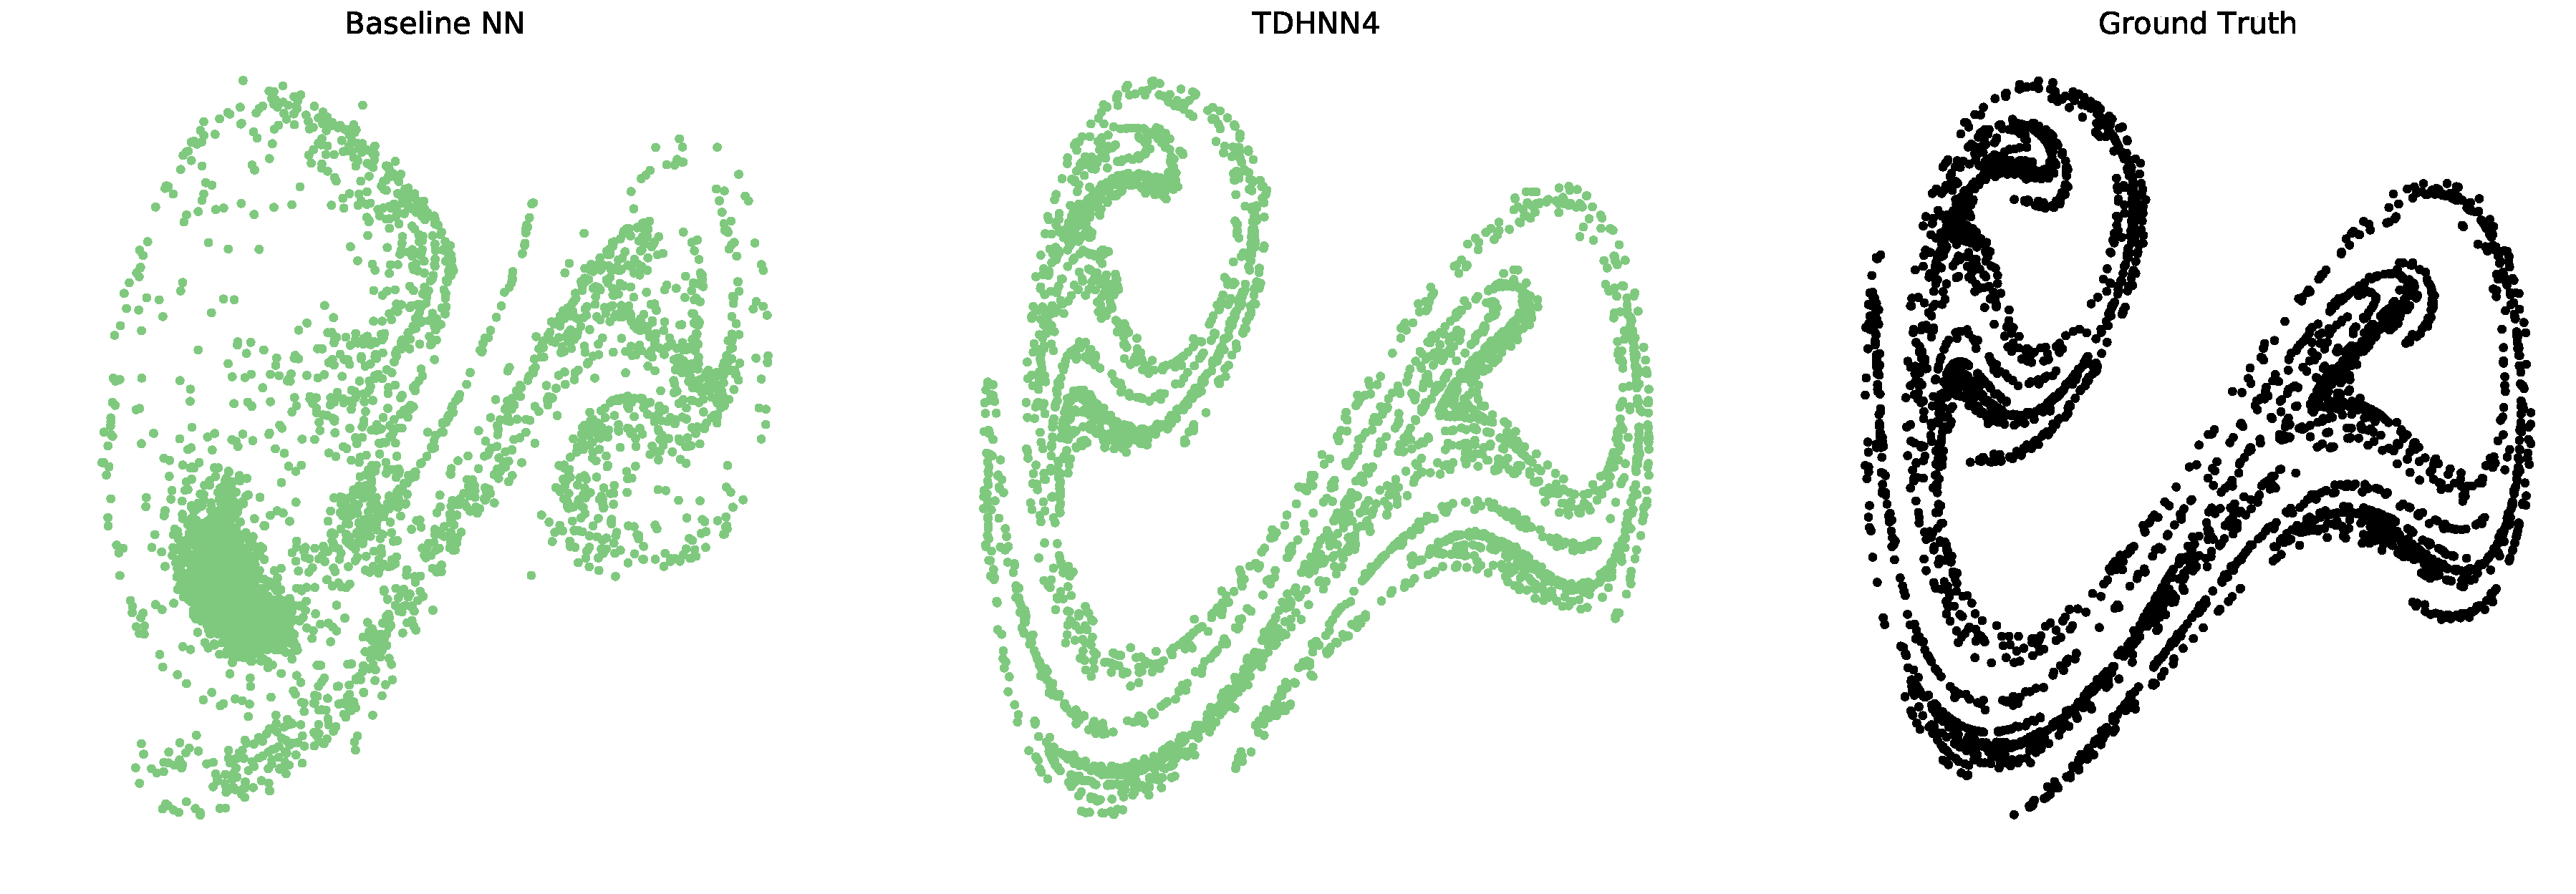
\includegraphics[width=0.9\textwidth]{figures/main_fig.pdf}
\caption{Poincar\'e Sections of a Duffing oscillator in a chaotic regime. Both Baseline NN and pHNN are trained for 20000 iterations with 2000 data points. pHNN significantly outperforms Baseline NN at recovering the ground truth Poincar\'e section of a test point not in the training set.}
\label{fig.chaos1}
\end{figure*}

\section{Introduction}

Neural networks (NNs), as universal function approximators \cite{hornik_multilayer_1989}, have shown resounding success across a host of domains including image segmentation \cite{he_mask_2018}, machine translation \cite{devlin_bert_2019} and even material property predictions \cite{toussaint_differentiable_2018,yao_tensormol-01_2018}. However, their performance in learning dynamical systems that obey physical laws has often been limited \cite{greydanus_hamiltonian_2019,pukrittayakamee_simultaneous_2009}. New research in \textit{scientific machine learning} - a field that tackles scientific problems with domain-specific machine learning methods, is paving a way to address this challenge. More specifically, it has been shown that physically-informed inductive biases embedded in networks, such as Hamiltonian mechanics \cite{mattheakis_hamiltonian_2020, greydanus_hamiltonian_2019}, Lagrangians \cite{cranmer_lagrangian_2020, lutter_deep_2019}, Ordinary Differential Equations (ODEs) \cite{chen_neural_2018}, physics-informed networks \cite{raissi_physics_2017} and Graph Neural Networks \cite{battaglia_interaction_2016,sanchez-gonzalez_hamiltonian_2019} can significantly improve learning over vanilla neural networks in complex physical domains. Furthermore, it has also been shown that such systems can be adapted to learn trajectories of controlled systems \cite{lutter_deep_2019,zhong_dissipative_2020}. 

Despite this extensive research, there is no method that accounts for explicit-time dependence, a crucial component in forced dynamical systems. Additionally, many of the existing approaches do not outline how to account for energy dissipation. In the present work, we outline how a Port-Hamiltonian formalism can be used to represent a forced and damped dynamical system. We then show how the underlying structure of this formalism can be embedded into a neural network in order to learn the dynamics of explicit time-dependent physical systems for which the forcing and damping terms are unknown apriori. We extensively benchmark our network on a range of tasks including the simple mass-spring system undergoing damping and complex forcing, the Duffing equation in both the non-chaotic and chaotic regimes as well as the Duffing equation for a relativistic particle. Our proposed network consistently outperforms other approaches while recovering both the driving force and the damping coefficient - an important result in system identification. Furthermore, we show that our network can be used to visually recover the Poincar\'e Section of the Duffing equation in a chaotic regime, a deeply promising result that can help us identify and understand chaotic trajectories (see Fig. \ref{fig.chaos1}).

\section{Background}

\subsection{Hamiltonian Neural Networks}

Recently, the authors of \cite{greydanus_hamiltonian_2019} demonstrate that the dynamics of an energy conserving autonomous system can be accurately learned by guiding a neural network to predict a Hamiltonian - an important representation of a dynamical system that generalizes classical mechanics. Considering dynamical systems of $M$ objects, the Hamiltonian $\mathcal{H}$ is a scalar function of a position vector $\mathbf{q}(t) = (q_1(t),q_2(t),....,q_M(t))$ and momentum vector $\mathbf{p}(t) = (p_1(t),p_2(t),....,p_M(t))$ that obeys Hamilton's equations,
\begin{equation}
\dot{\mathbf{q}}= \frac{\partial \mathcal{H}}{\partial \mathbf{p}}, ~~~
\dot{\mathbf{p}}= -\frac{\partial \mathcal{H}}{\partial \mathbf{q}},
\label{eqn.hamiltonian}
\end{equation}
where $\dot{\mathbf{q}}=\frac{d\mathbf{q}}{dt}$ and  $\dot{\mathbf{p}}=\frac{d\mathbf{p}}{dt}$. In the following, we drop the time dependence where the context makes it clear.

Using this formalism, \cite{greydanus_hamiltonian_2019} 
show that a neural network, parametrized by $\theta$, can be used to learn a scalar output Hamiltonian $H_{\theta}(\mathbf{q},\mathbf{p})$ given $\mathbf{q}$ and $\mathbf{p}$ as inputs to the network. Using this predicted Hamiltonian, it is possible to recover the time derivatives of the input by simply differentiating (via autograd) the Hamiltonian with respect to its inputs. The derivatives of the Hamiltonian $\left [ \frac{\partial \mathcal{H}}{\partial \mathbf{p}},-\frac{\partial \mathcal{H}}{\partial \mathbf{q}} \right ]$ provide us with time derivatives of the input state vector $[\dot{\mathbf{q}},\dot{\mathbf{p}}]$. Therefore, once trained, this network yields an approximate time derivative generator for the state $[\mathbf{q},\mathbf{p}]$ and as such can be used in a numerical integrator to evolve an initial condition $[\mathbf{q}_t,\mathbf{p}_t]$, as in Eq.\ref{eqn.action_int}.
\begin{equation}
(\mathbf{q},\mathbf{p})_{t+1} = (\mathbf{q},\mathbf{p})_t + \int_t^{t+1} \left [ \frac{\partial \mathcal{H}}{\partial \mathbf{p}},-\frac{\partial \mathcal{H}}{\partial \mathbf{q}} \right ] \mathrm{d}t.
\label{eqn.action_int}
\end{equation}
In addition, the vector field $\mathbf{S} = \left [ \frac{\partial \mathcal{H}}{\partial \mathbf{p}},-\frac{\partial \mathcal{H}}{\partial \mathbf{q}} \right ]$ is a symplectic gradient. This means that $\mathcal{H}$ remains constant as long as the state vectors are integrated along $\mathbf{S}$. This result links the Hamiltonian with the total energy of the system such that $\mathcal{H}(\mathbf{q},\mathbf{p}) = E_{\mathrm{tot}}$ for many autonomous physical systems. Therefore, the Hamiltonian is a powerful inductive bias that can be utilized to evolve a physical state while maintaining energy conservation. It is precisely for this reason that HNN outperforms traditional approaches that directly predict the state time derivatives from the input state. However, this formulation does not readily generalize to damped or forced time-varying systems.

\subsection{Port-Hamiltonians}

The Port-Hamiltonian \cite{sanz-sole_port-hamiltonian_2007,acosta_interconnection_2005,zheng_time-varying_2018,cherifi_overview_2020} is a well studied formalism in control literature that allows us to generalize Hamilton's equations to incorporate energy dissipation and an external control input to a dynamical system. A recent method that embeds the Port-Hamiltonian in a neural network \cite{zhong_dissipative_2020} shows how to represent a general form for such a system. In \cite{zhong_dissipative_2020} the Port-Hamiltonian is represented as:
\begin{equation}
\resizebox{0.9\linewidth}{!}{$%
\begin{bmatrix}
\dot{\mathbf{q}} \\
\dot{\mathbf{p}}
\end{bmatrix}
=
\Bigg(\begin{bmatrix}
\mathbf{0} & \mathbf{I} \\
-\mathbf{I} & \mathbf{0}
\end{bmatrix} +
\mathbf{D}(\mathbf{q})
 \Bigg)
 \begin{bmatrix}
\frac{\partial \mathcal{H}}{\partial \mathbf{q}} \\
\frac{\partial \mathcal{H}}{\partial \mathbf{p}}
\end{bmatrix}
+
\begin{bmatrix}
\mathbf{0} \\
\mathbf{G}(\mathbf{q})
\end{bmatrix}
\mathbf{u},
$%
}%
\label{eqn.pham}
\end{equation}
where $\mathbf{D}(\mathbf{q})$ is a matrix to account for damping and $\mathbf{G}(\mathbf{q})\mathbf{u}$ is an external control term where $\mathbf{u}$ is a temporal control input and $\mathbf{G}(\mathbf{q})$ is a spatial matrix. $\mathbf{I}$ is the identity matrix and $\mathbf{0}$ the zero matrix. In this setting, the vector $[\mathbf{q},\mathbf{p},\mathbf{u}]$ is provided as input to the system. The matrix $\mathbf{D}(\mathbf{q})$ is assumed to be semi-positive definite and $\mathbf{G}(\mathbf{q})$ is typically a non-linear scaling of $\mathbf{q}$. This general formalism allows us to collapse to a classical Hamiltonian system by simply setting $\mathbf{D}$ and $\mathbf{u}$ to zero. Typically, the Port Hamiltonian is used in control applications where explicit knowledge of the control term $\mathbf{u}$ is known, however, in this paper we explore an adaptation of this formalism in which we do not know the control term and make this a learnable function. We do this because in some applications, it might be useful to uncover/identify to underlying forcing term from the state vector where no explicit knowledge of the control input is available. 

\section{Related Work}

While Hamiltonian mechanics presents one way to address learning dynamical systems, numerous recent methods highlight how incorporating physically-informed inductive biases into neural networks can improve learning.

\subsection*{Functional Priors}
Functional priors, for example, embed the full functional form of an equation into the neural network. Physics-informed Neural Networks (PINNs) \cite{raissi_physics_2017,raissi_physics-informed_2019} and Hamiltonian Nets \cite{mattheakis_hamiltonian_2020} are two such approaches that look at directly embedding the equations of motion into the loss function. While PINNs are data-driven approaches that rely on autograd to compute partial-derivatives of a hidden state, Hamiltonian Nets are data-independent approaches that pre-specify the full functional form of a system-specific Hamiltonian in the loss function.

\subsection*{Integrator Priors}
Many recent methods have sought to use a NN to parametrize the time derivatives of a state vector and then use this learned parametrization in a numerical integrator such as a Runge-Kutta method. The authors of NeuralODE \cite{chen_neural_2018} show that embedding the integrator into the learning process induces a continuous depth neural network for large time-step predictions. As such, the number of gradient computations scales exponentially with the number of integrative time steps during backpropagation through the integrator. The authors of NeuralODE thus show that the adjoint method can be used to ensure linear scaling of the gradient computations. More recent work has looked at generalizing this approach to different topologies that classical NeuralODEs cannot represent \cite{dupont_augmented_2019}. Other work such as \cite{zhu_deep_2020}, theoretically shows the importance of using symplectic integrators over Runge-Kutta methods to evolve Hamiltonian systems in NNs.

\subsection*{Graph based methods}
In \cite{battaglia_interaction_2016}, the authors detail how a Graph Neural Network, designed to capture the relational structure of systems, can be used to learn interacting particle systems. This work has been exploited in numerous advances \cite{sanchez-gonzalez_graph_2018,sanchez-gonzalez_learning_2020,cranmer_lagrangian_2020} and emphasizes how a relation inductive bias can significantly improve learning.

\subsection*{Lagrangian/Hamiltonian Methods}
While \cite{cranmer_lagrangian_2020} and \cite{greydanus_hamiltonian_2019} propose to explicitly learn Hamiltonian and Lagrangian functions, \cite{lutter_deep_2019} shows how one can exploit the Lagrangian equation to learn both a function which can predict the generalized forces as well as use generalized forces and coordinate information to predict the next state. The authors show that their inverse model can accurately predict a controlled double pendulum, which is pertinent for controlled robots.

\subsection*{Latest Advances}
Recent work studies Constrained HNN \cite{finzi_generalizing_2020}, an approach that looks at enforcing Cartesian coordinates in Hamiltonians and Lagrangians with holonomic constraints. The paper emphasises that such a framework works significantly better at learning deeply complex physical systems such as the 5-pendulum. 

Despite these significant breakthroughs, there is no existing method that investigates explicit time-dependence and damping in such systems, elements that are often found in real world problems. As such, we outline a novel technique to address this challenge.

\section{Method}

\subsection{Theory}
Our method, Time Dependent Port Hamiltonian NN (pHNN), takes the form of the Port-Hamiltonian with two modifications. First, our approach exploits the fact that many damped systems consist of a non-zero, state-independent damping term in the lower right quadrant, so we replace the damping matrix $\mathbf{D}(\mathbf{q})$ with a state independent lower right matrix $\mathbf{N}$. Secondly, in order to generalize to time dependent forcing, we replace $\mathbf{G}(\mathbf{q})\mathbf{u}$ with $\mathbf{F}(t)$. The resulting representation, as highlighted in Eq.(\ref{eqn.pham1}), is now general enough to handle many well-known forced systems but also specific enough to tackle learning in physical domains of practical importance such as the Duffing equation.
\begin{equation}
\resizebox{0.9\linewidth}{!}{$%
\begin{bmatrix}
\dot{\mathbf{q}} \\
\dot{\mathbf{p}}
\end{bmatrix}
=
\Bigg(\begin{bmatrix}
\mathbf{0} & \mathbf{I} \\
-\mathbf{I} & \mathbf{0}
\end{bmatrix} +
\begin{bmatrix}
\mathbf{0} & \mathbf{0} \\
\mathbf{0} & \mathbf{N}
\end{bmatrix}
 \Bigg)
 \begin{bmatrix}
\frac{\partial \mathcal{H}}{\partial \mathbf{q}} \\
\frac{\partial \mathcal{H}}{\partial \mathbf{p}}
\end{bmatrix}
+
\begin{bmatrix}
\mathbf{0} \\
\mathbf{F}(t)
\end{bmatrix}.
$%
}%
\label{eqn.pham1}
\end{equation}
\begin{figure}[h!]
\centering
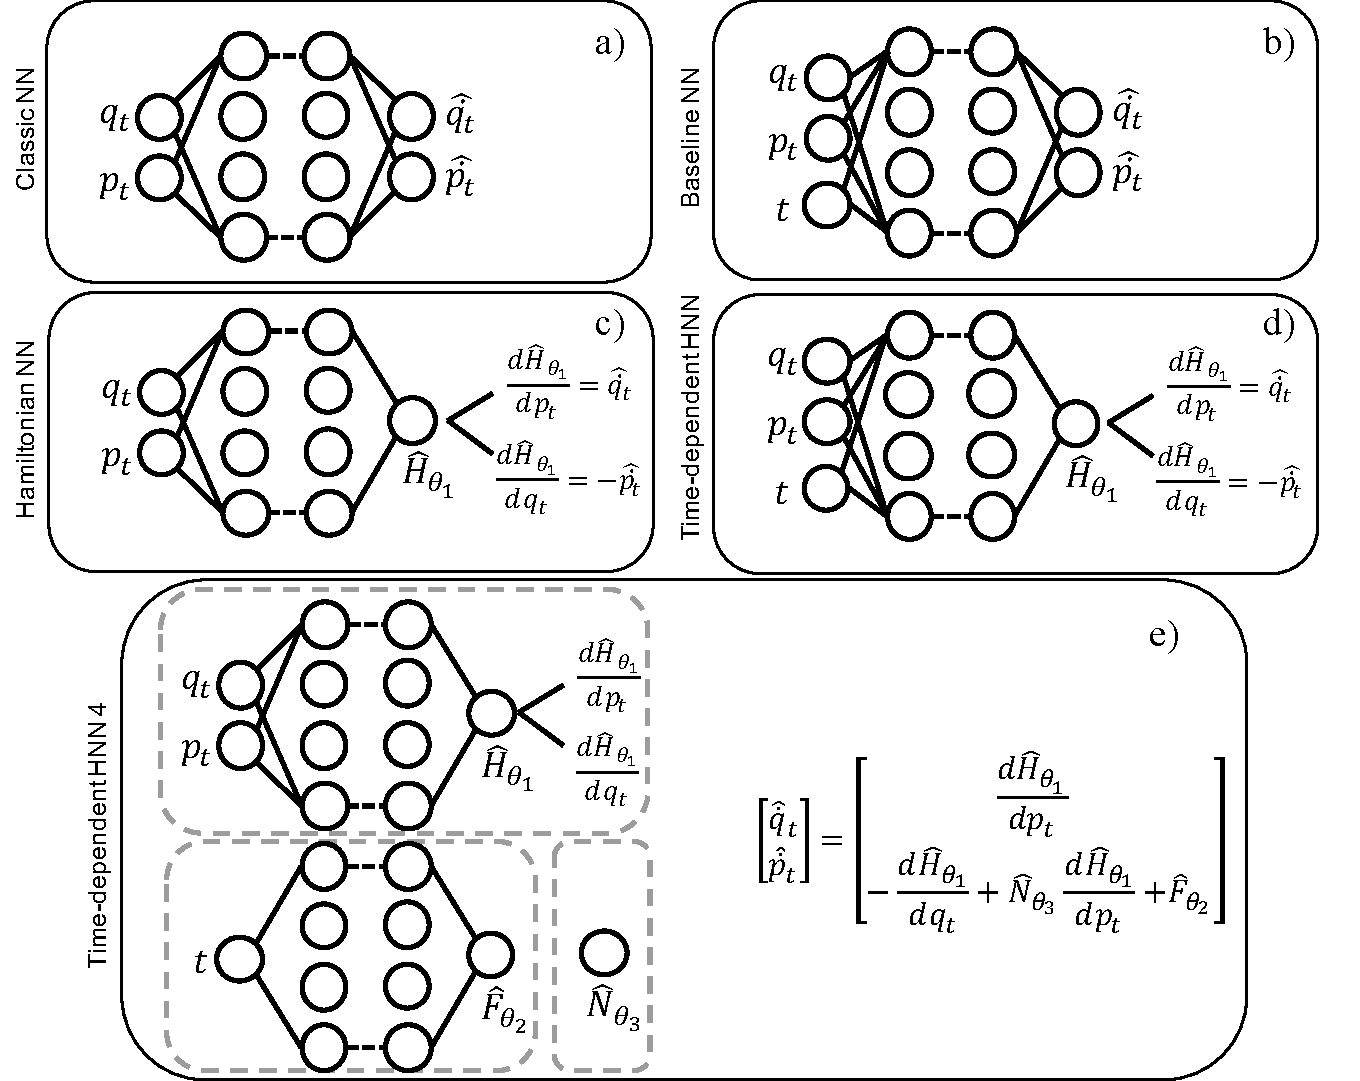
\includegraphics[width=0.5\textwidth]{figures/architecture2.pdf}
\caption{Architectures used to learn dynamics in this paper. The naive extension of classic NN (a) and Hamiltonian NN (c) is to incorporate time as an additional input variable (b and d). Our innovation, which exploits Port-Hamiltonians, explicitly learns the force $F_{\theta_2}$ as well as the damping term $N_{\theta_3}$ (e).}
\label{fig.architecture}
\end{figure}
The architecture for our method as well as existing approaches are shown in Fig.\ref{fig.architecture}. Classic NN Fig.\ref{fig.architecture}(a) and Hamiltonian NN Fig.\ref{fig.architecture}(c) \cite{greydanus_hamiltonian_2019} simply take position and momentum as inputs and are designed to yield the time derivatives of the input, with HNN learning an intermediary Hamiltonian and employing backpropagation to compute the output. One natural way to extend these architectures for time-varying non-autonomous systems is to simply include time as an additional input. This readily gives rise to Baseline NN (Fig.\ref{fig.architecture}(b)) and Time-Dependent HNN (Fig.\ref{fig.architecture}(d)). While we will see that both these approaches are reasonable, they do not help us identify the underlying force or damping terms, nor are they consistently performant across the applications we investigate. Our network Fig.\ref{fig.architecture}(e) goes beyond this naive approach and embeds the Port-Hamiltonian. The network is designed to learn the Hamiltonian, $\mathcal{H}$, the driving force, $\mathbf{F}$, and the damping term, $\mathbf{N}$, and combine these to obtain estimates of the state time derivatives. 

\subsection{Training}
To train the network, we feed in $ [\mathbf{q},\mathbf{p},t]$ to our model. The first component, $\mathcal{H}_{\theta_1}$, consists of three hidden layers designed to predict $\mathcal{H}$ from $[\mathbf{q},\mathbf{p}]$ input data. The second component, $\mathbf{N}_{\theta_3}$, consists of a single weight parameter (i.e. $\theta_3$ is a single node) designed to learn the damping. The third neural-network consists of three hidden layers designed to predict $\mathbf{F}(t)$. The output of each component is combined as per Eq.\ref{eqn.pham1} to obtain predictions of the state time derivatives $[\hat{\dot{\mathbf{q}}},\hat{\dot{\mathbf{p}}}]$. Using these predictions, we define our loss function as:
\begin{equation}
\label{eqn.loss}
\resizebox{0.9\columnwidth}{!}{%
  $\mathcal{L} =|| \hat{\dot{\mathbf{q}}}_t - \dot{\mathbf{q}}_t ||_2^2 +
|| \hat{\dot{\mathbf{p}}}_t -\dot{\mathbf{p}}_t ||_2^2 + \lambda_F|| \hat{\mathbf{F}}_{\theta_2} (t)||_1 + \lambda_N||\hat{\mathbf{N}}_{\theta_3}||_1$.%
}
\end{equation}
The loss function minimizes the loss between the predicted and ground truth state time derivatives with a squared error loss. In addition, the forcing and damping terms are added to the loss with an L1 penalty when using pHNN. The latter choice is made to encourage the networks to learn simpler models. We also find, during experimentation, that this choice is superior to L2 in enabling us to identify the ground truth force and damping terms. The choice of hyper-parameters $\lambda_F$ and $\lambda_{N}$ is made via a grid search across $[10^{-2},10^{-4},10^{-6},10^{-8}]$, for each parameter, that generates the lowest validation loss (details in Appendix D). For our experiments we use 200 nodes per layer and find that most activations, including $\tanh$,$\sin$ and $\cos$ yield comparable results. 
\subsubsection{Training Dataset}

Training data is generated using a 4th order Runge-Kutta integrator. Several simulations were run with different initial conditions for $t\in [0,T_{\max}]$. At each iteration, the next state as well as the state derivatives are recorded. This is typically done for multiple initial conditions and then passed to the network for training. Details for how initial conditions are sampled are described independently for each system in the results section.

\subsection{Testing}
Once trained, each of the networks in Fig.\ref{fig.architecture} can approximate $[\dot{\mathbf{q}},\dot{\mathbf{p}}]$. As such, they can be used in a scientific integrator such as a Runge-Kutta 4th order method to integrate initial conditions not in the training dataset from $t=0$ to $t=T_{\max}$ which we refer to as a state rollout. We measure the performance of the network by comparing the predicted state rollout with the ground truth. We do this by computing a mean squared error across the state variables and across time. Therefore:
\begin{equation}
\resizebox{0.9\linewidth}{!}{$%
\mathrm{MSE}_{\mathrm{state}} = \frac{1}{2N} \left(\sum_{i=1}^N (\mathbf{q}_i-\hat{\mathbf{q}}_i)^2 + \sum_{i=1}^N (\mathbf{p}_i - \hat{\mathbf{p}}_i)^2\right),$}%
\end{equation}
and
\begin{equation}
\resizebox{0.9\linewidth}{!}{$%
\mathrm{MSE}_{\mathrm{energy}} = \frac{1}{N} \sum_{i=1}^N \left(\mathcal{H}(\mathbf{q}_i,\mathbf{p}_i)-\mathcal{H}(\hat{\mathbf{q}}_i,\hat{\mathbf{p}}_i)\right)^2$}%
\end{equation}
where $N = T_{\max}/\Delta t $, with $\Delta t$ as the integrative step. We typically compute these terms for multiple different initial conditions during inference and average across them (see Fig.\ref{mspring}(c)).

\subsection{Procedure}

\begin{enumerate}
\item Obtain state variable data $[\mathbf{q},\mathbf{p},t]$ and time derivatives $[\dot{\mathbf{q}},\dot{\mathbf{p}}]$ from trajectories of a given system.
\item Provide state-variable information to pHNN which learns a Hamiltonian, force and damping term to predict $[\hat{\dot{\mathbf{q}}},\hat{\dot{\mathbf{p}}}]$.
\item Minimize predictions with ground truth time-derivatives as in Eqn.(\ref{eqn.loss}).
\item Once trained, use the network as a time-derivative generator in a scientific integrator to integrate a set of initial conditions $[\mathbf{q}_0,\mathbf{p}_0]$ to $[\mathbf{q}_T,\mathbf{p}_T]$.
\end{enumerate}

\section{Results}

We benchmark the performance of our models on numerous datasets that cover time-independent systems to complex chaotic forced systems. The results are presented in order of increasing complexity from a model perspective.

\subsection{Simple Mass-Spring System}

We begin our analysis with a simple mass-spring system, obeying Hooke's Law from classical physics with no force or damping. The Hamiltonian is,
\begin{equation}
\mathcal{H} = \frac{1}{2}kq^2 + \frac{1}{2m}p^2. 
\end{equation}
where $k$ is the spring constant and $m$ is the mass of the object. Note, the position and moment are scalars.

\textbf{Training:} Without loss of generalization, we set $k$ and $m$ to 1 for our experiments. We randomly sample 25 initial training conditions $[q_0,p_0]$ that satisfy $q_0^2+p_0^2 = r_0^2$ where $1 \leq r_0 \leq 4.5$ which corresponds to sampling initial conditions with energies between 1 and 4.5. We integrate each using a 4th order RK method with $\Delta t =0.05$ and $T_{\max} = 3.05$. 

\textbf{Test:} At test time, we sample 25 initial conditions, not in the training set, and evolve them to $T_{\max}=3.05$. We investigate this simple system to show that learning a separate, regularized forcing term results in much better state and energy predictions in comparison to TDHNN and the Baseline NN which may not readily ignore the time variable fed in. Learning a separate forcing term and regularizing it keeps the time component independent of the Hamiltonian and therefore allows us to closely match the performance of classical time-implicit HNN. 

\begin{figure}[h!]
\centering
%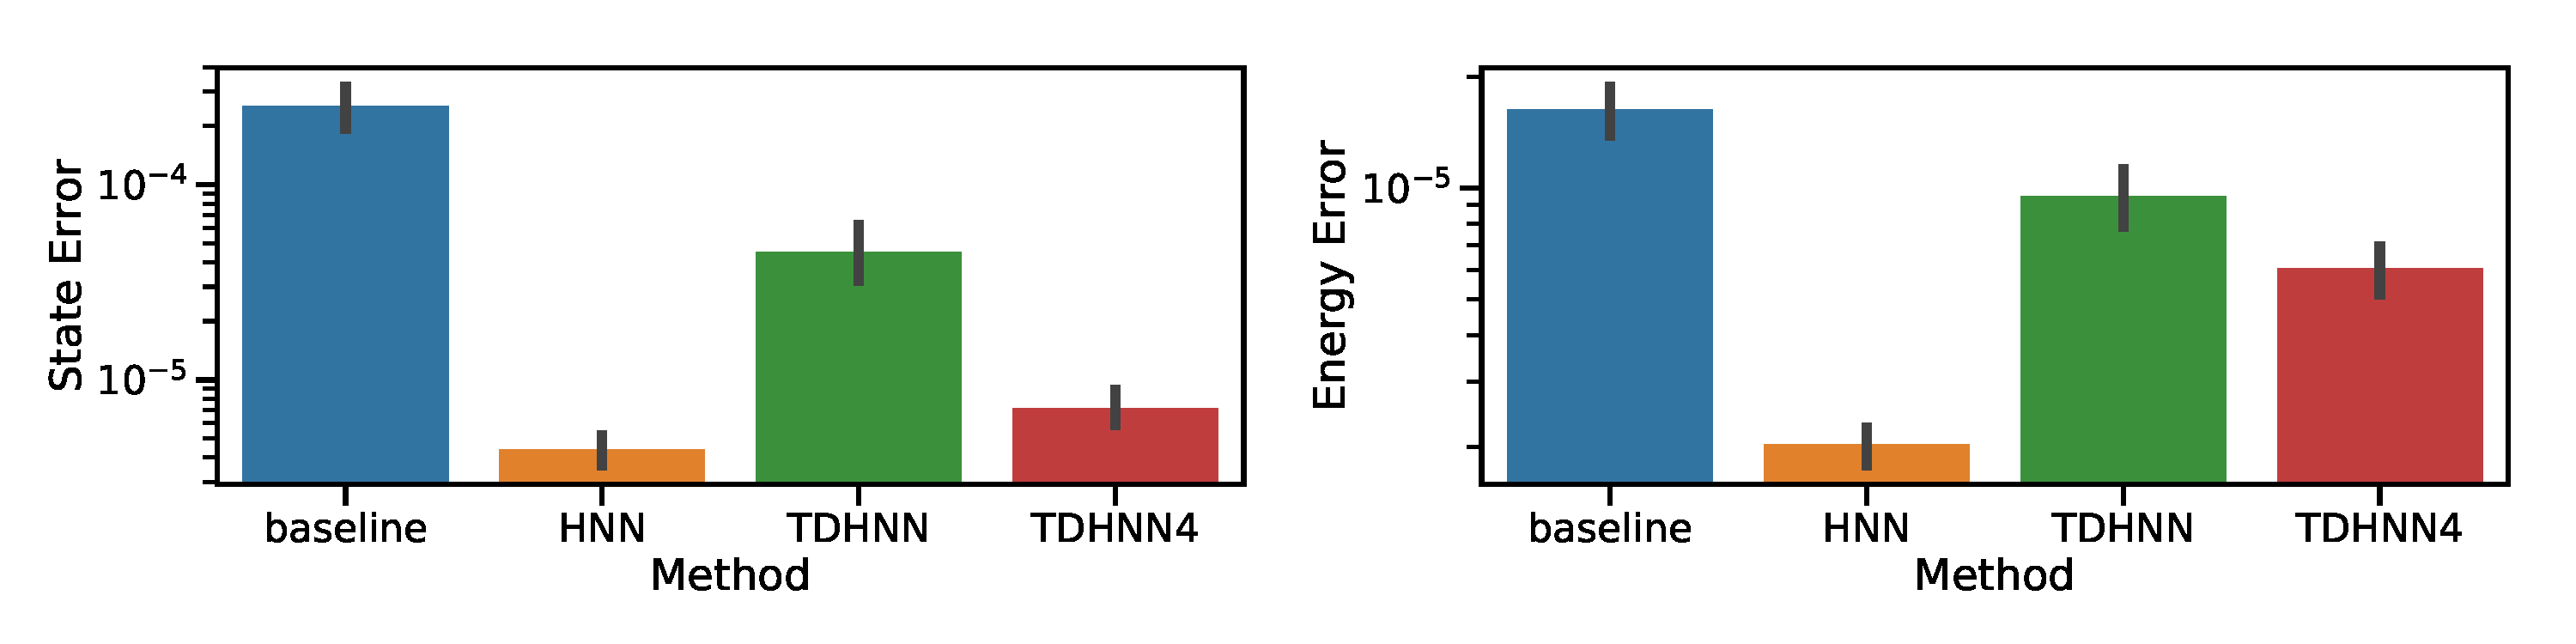
\includegraphics[width=0.4\textwidth]{figures/mass_spring_errors.pdf}
\captionsetup{justification=centering}
	\begin{subfigure}[b]{0.4\textwidth}
		\centering
		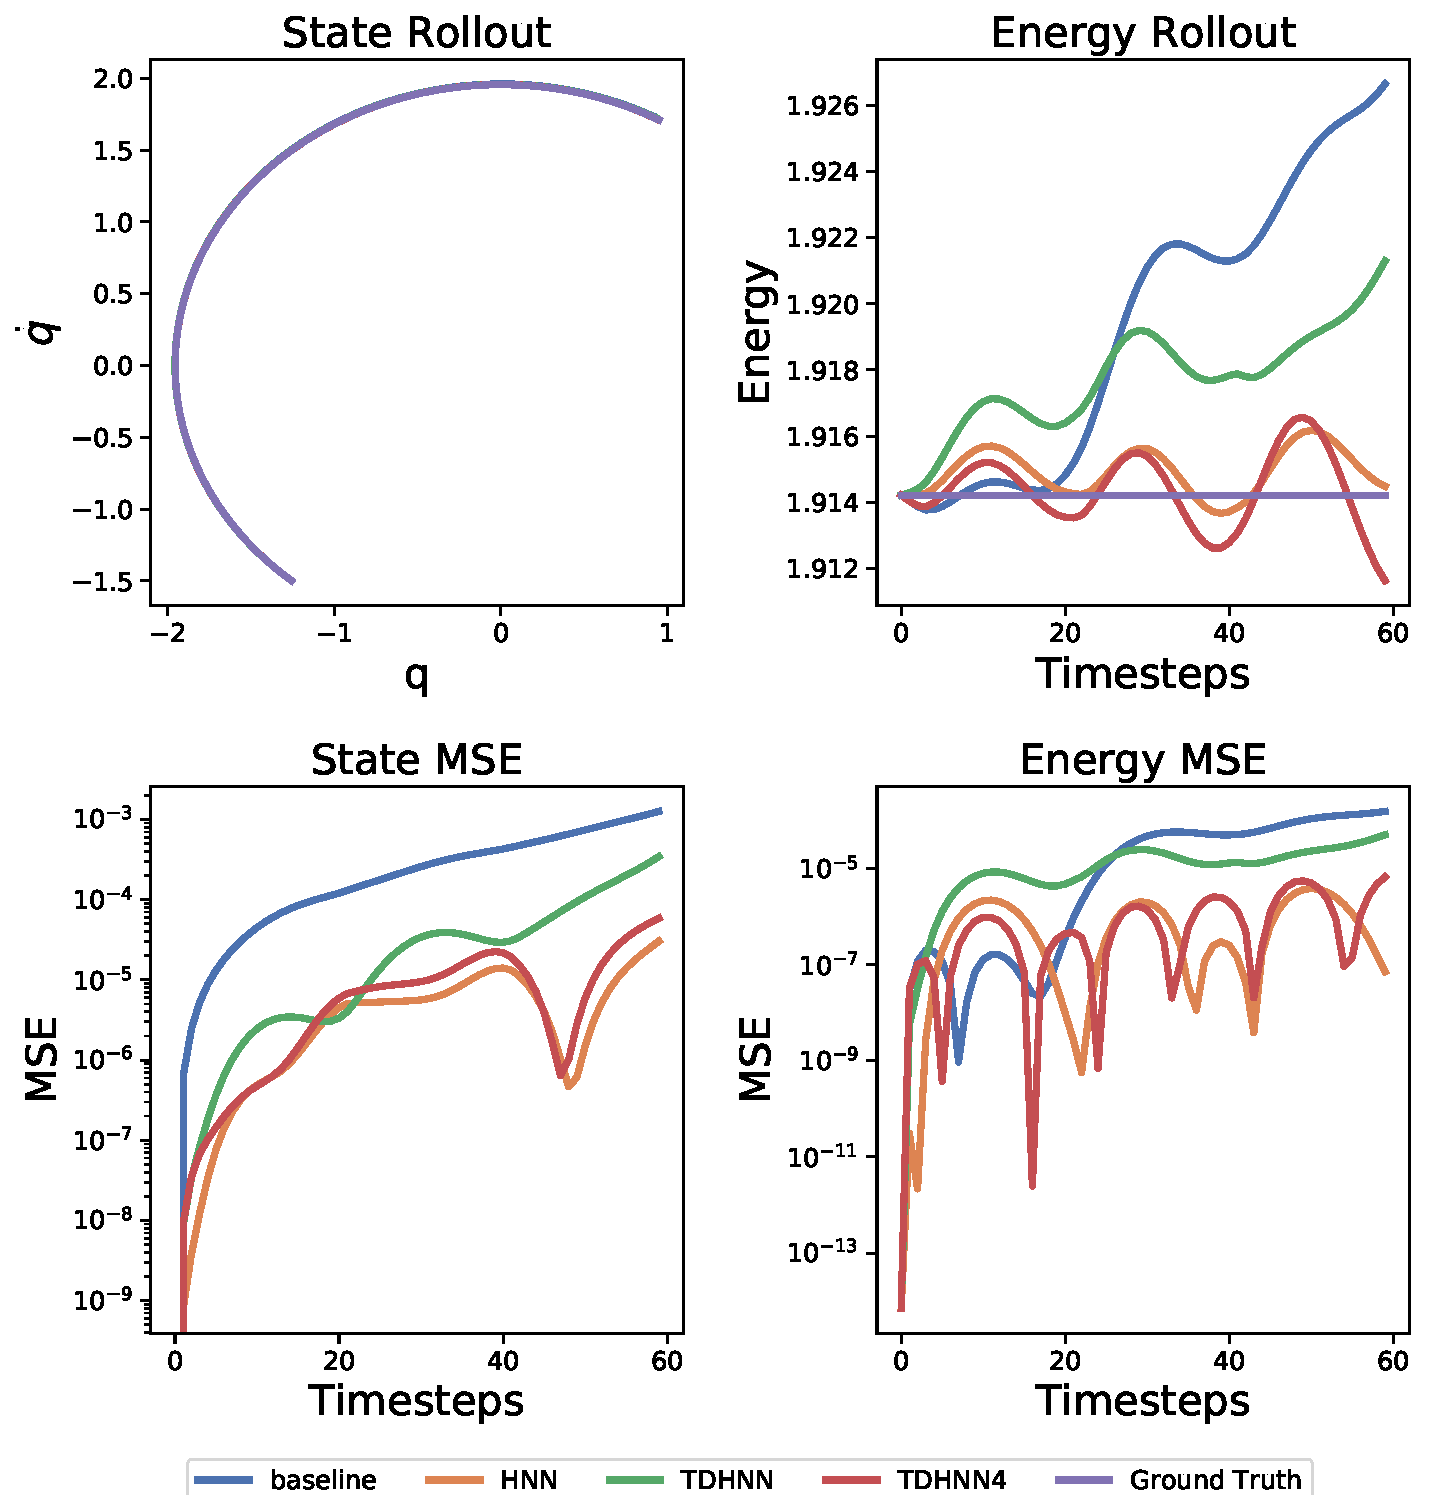
\includegraphics[width=\textwidth, trim={0 0 0 12cm},clip]{figures/figures/mass_spring/1/mass_spring_long_0.pdf}
		\caption{State and energy MSE as a function of time of an initial condition in the test set.}
	\end{subfigure}
	\begin{subfigure}[b]{0.48\textwidth}
		\centering
		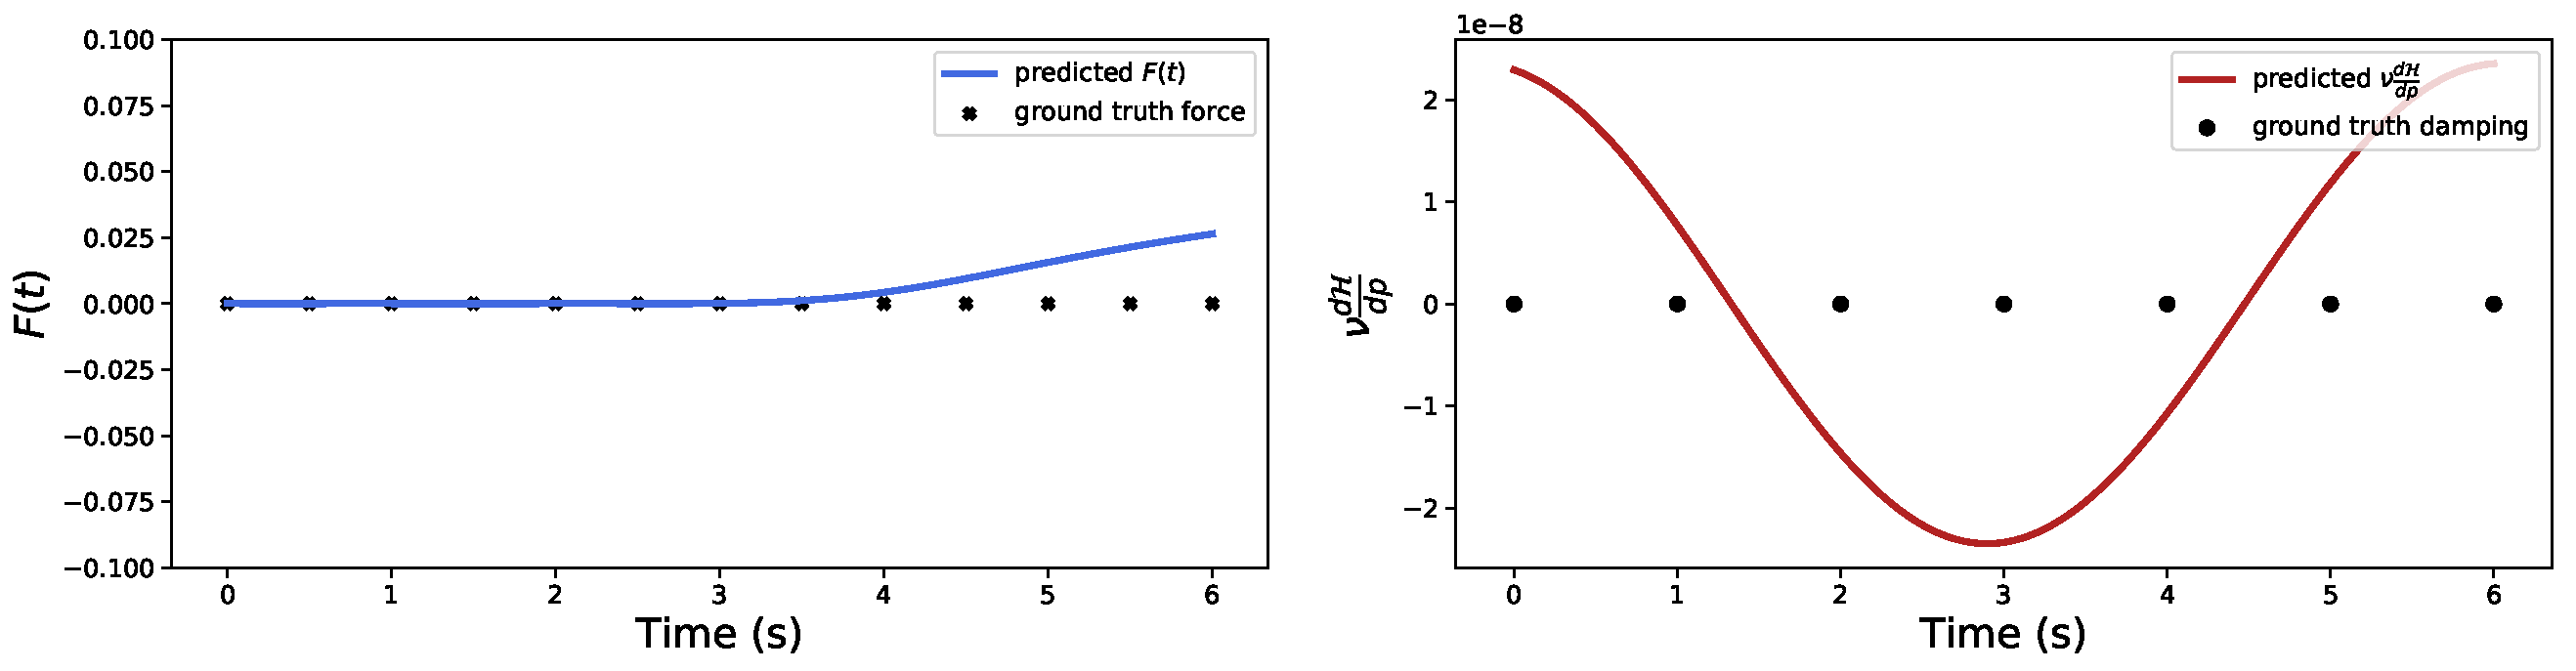
\includegraphics[width=\textwidth]{figures/figures/mass_spring/1/mass_spring_dpdt_new_0.pdf}
		\caption{Learnt force and damping terms by pHNN}
	\end{subfigure}
	\begin{subfigure}[b]{0.48\textwidth}
	    \centering
		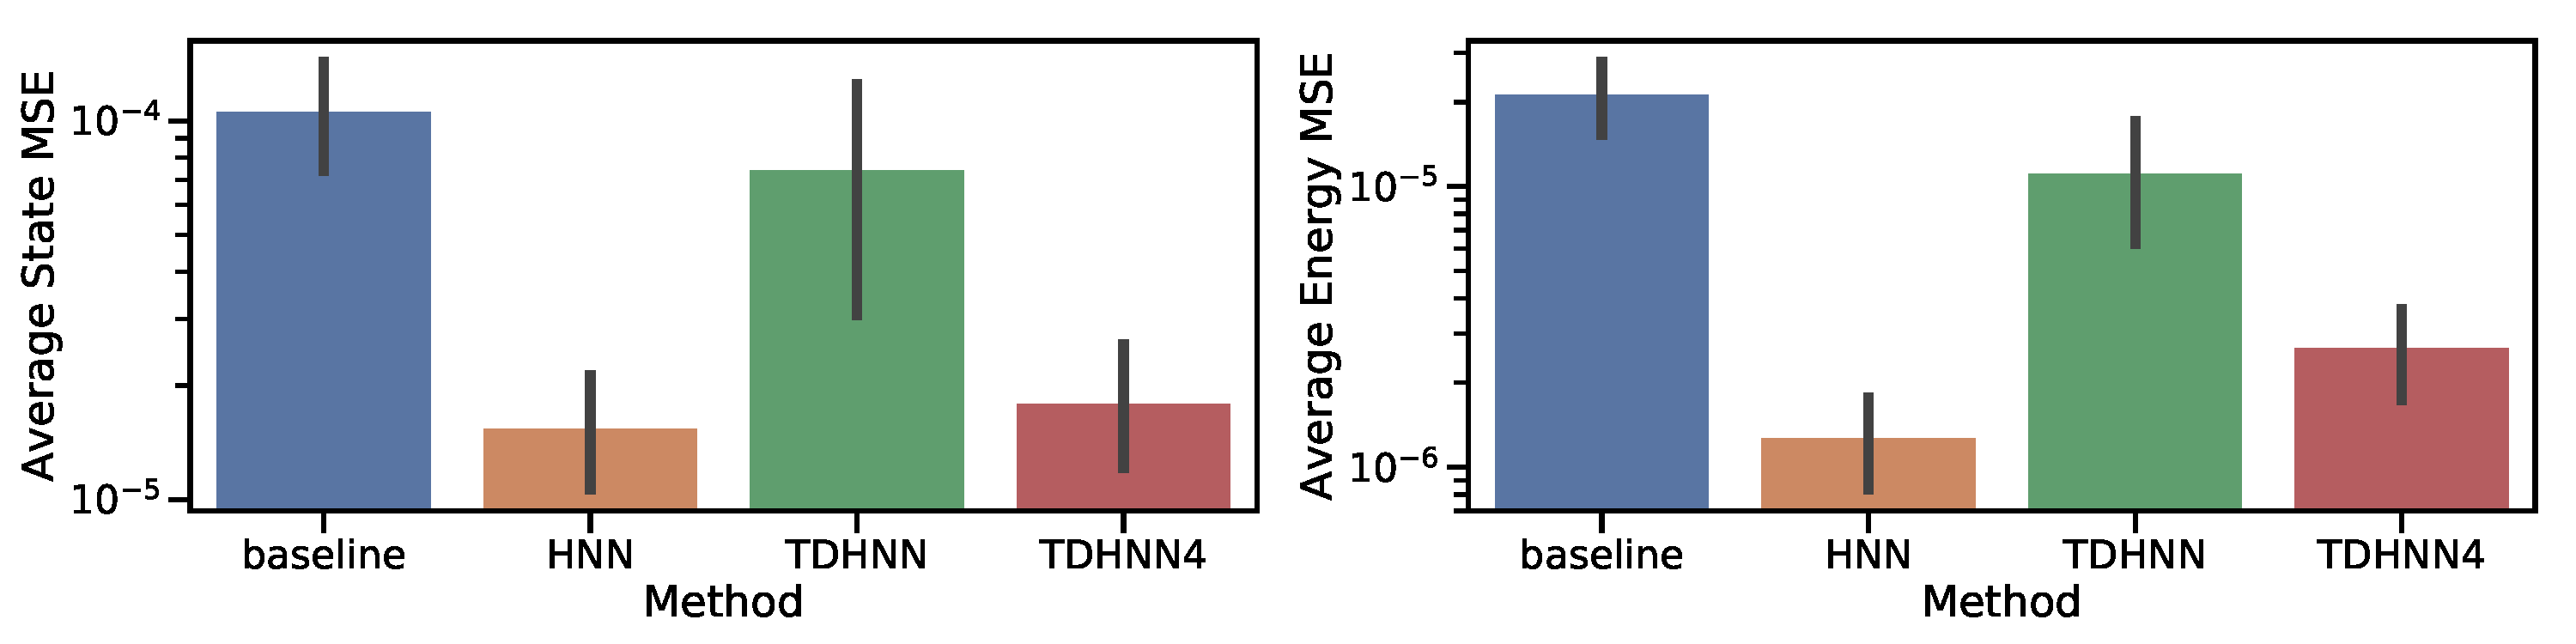
\includegraphics[width=\textwidth]{figures/figures/mass_spring/1/mass_spring_errors_0.pdf}
		\caption{State and energy MSE averaged across 25 initial test states}
	\end{subfigure}
\caption{The simple mass-spring system has no explicit time dependence. We see that pHNN can almost recover the dynamics as well as in HNN. The baseline NN and TDHNN are unable to achieve the same test state error as they are only reliable for time steps that are within the training regime. While pHNN does learn a non-zero force and damping term, their contribution to $\frac{dp}{dt}$ is small.}
\label{mspring}
\end{figure}

\subsection{Damped Mass-Spring System}

We extend the simple mass-spring system to include a damping term that reduces the initial energy of the system over time. The inclusion of this term violates energy conservation and therefore we cannot write a scalar Hamiltonian for such a system (see Appendix A.1 for details). Knowing this apriori already gives us an indication that HNN will perform poorly on such a system. The damped mass-spring system is typically used as a model to design shock absorbers for cars in order to ensure a smooth and safe ride. 

\textbf{Training:} We have 20 initial training conditions, with position and momentum uniformly sampled in $[-1,1]^2$. Each trajectory is evolved until $T_{\max} = 30.1$ with a $\Delta t = 0.1$. We fix the damping coefficient $\nu = 0.3$ without loss of generality to other coefficients.

\textbf{Test:} At inference, we compute the average rollout MSE of 25 unseen initial conditions sampled in the same manner as the training data, and report the average state and energy rollout MSE (see Fig.\ref{damped}).

\begin{figure}[h!]
\centering
\captionsetup{justification=centering}
%	\begin{subfigure}[b]{0.4\textwidth}
%		\centering
%		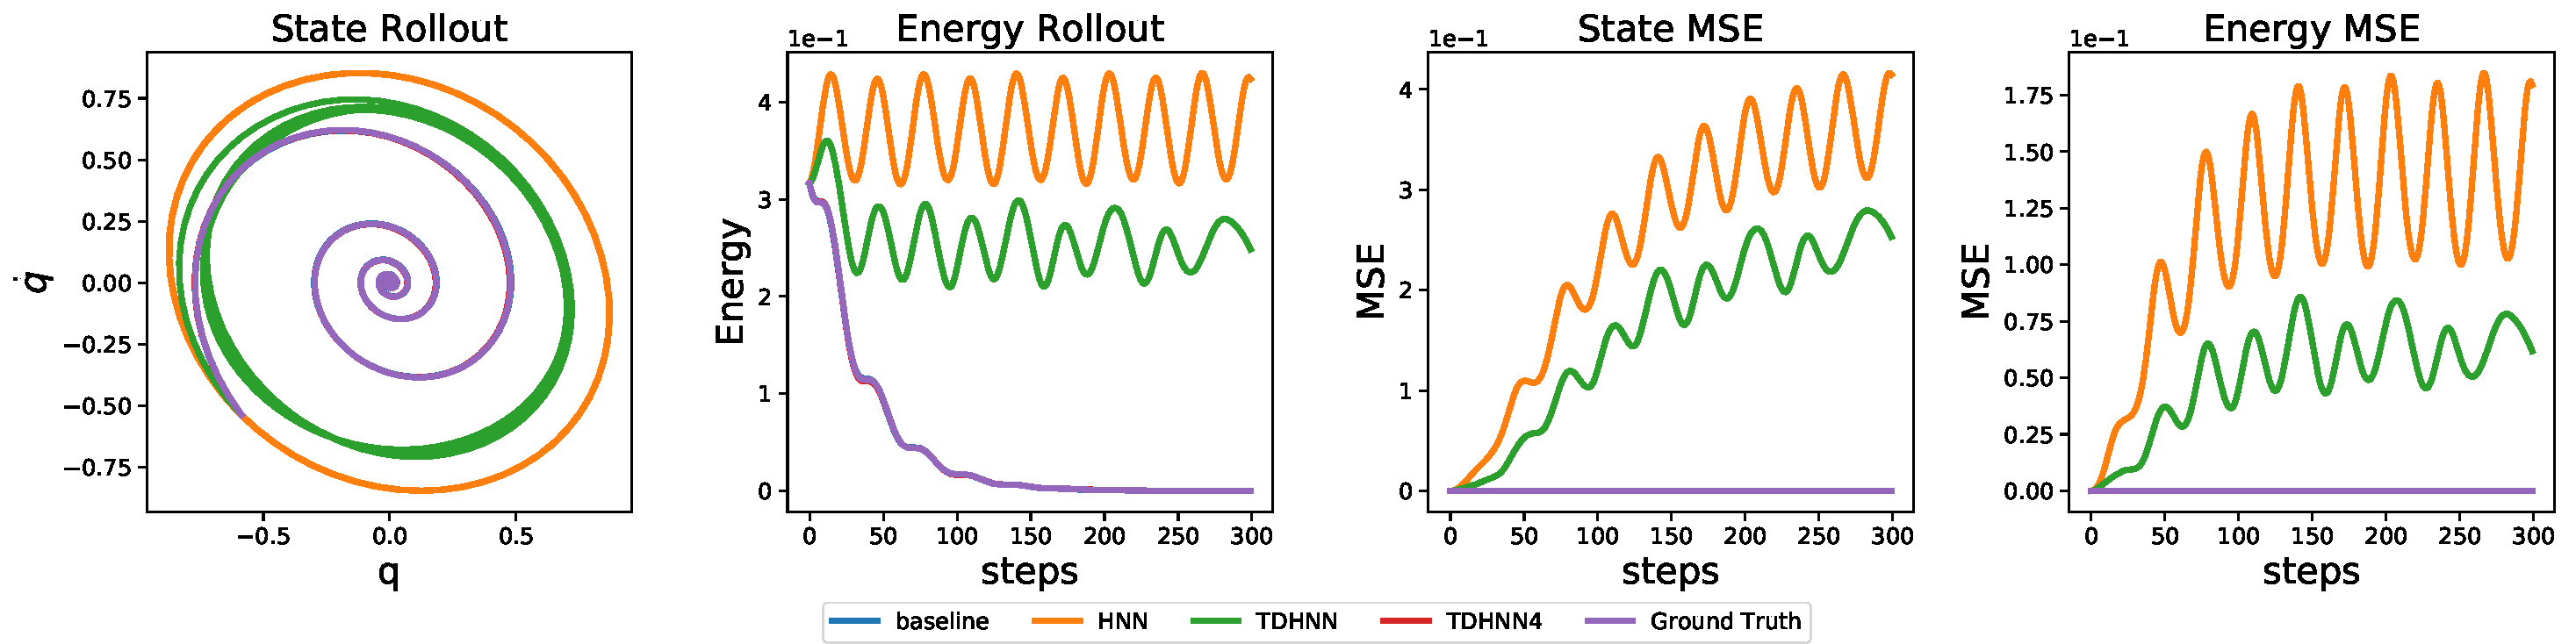
\includegraphics[width=\textwidth]{figures/damped_1_pred.pdf}
%		\caption{State and energy rollout/MSE of an initial condition in the test set.}
%	\end{subfigure}
	\begin{subfigure}[b]{0.48\textwidth}
		\centering
		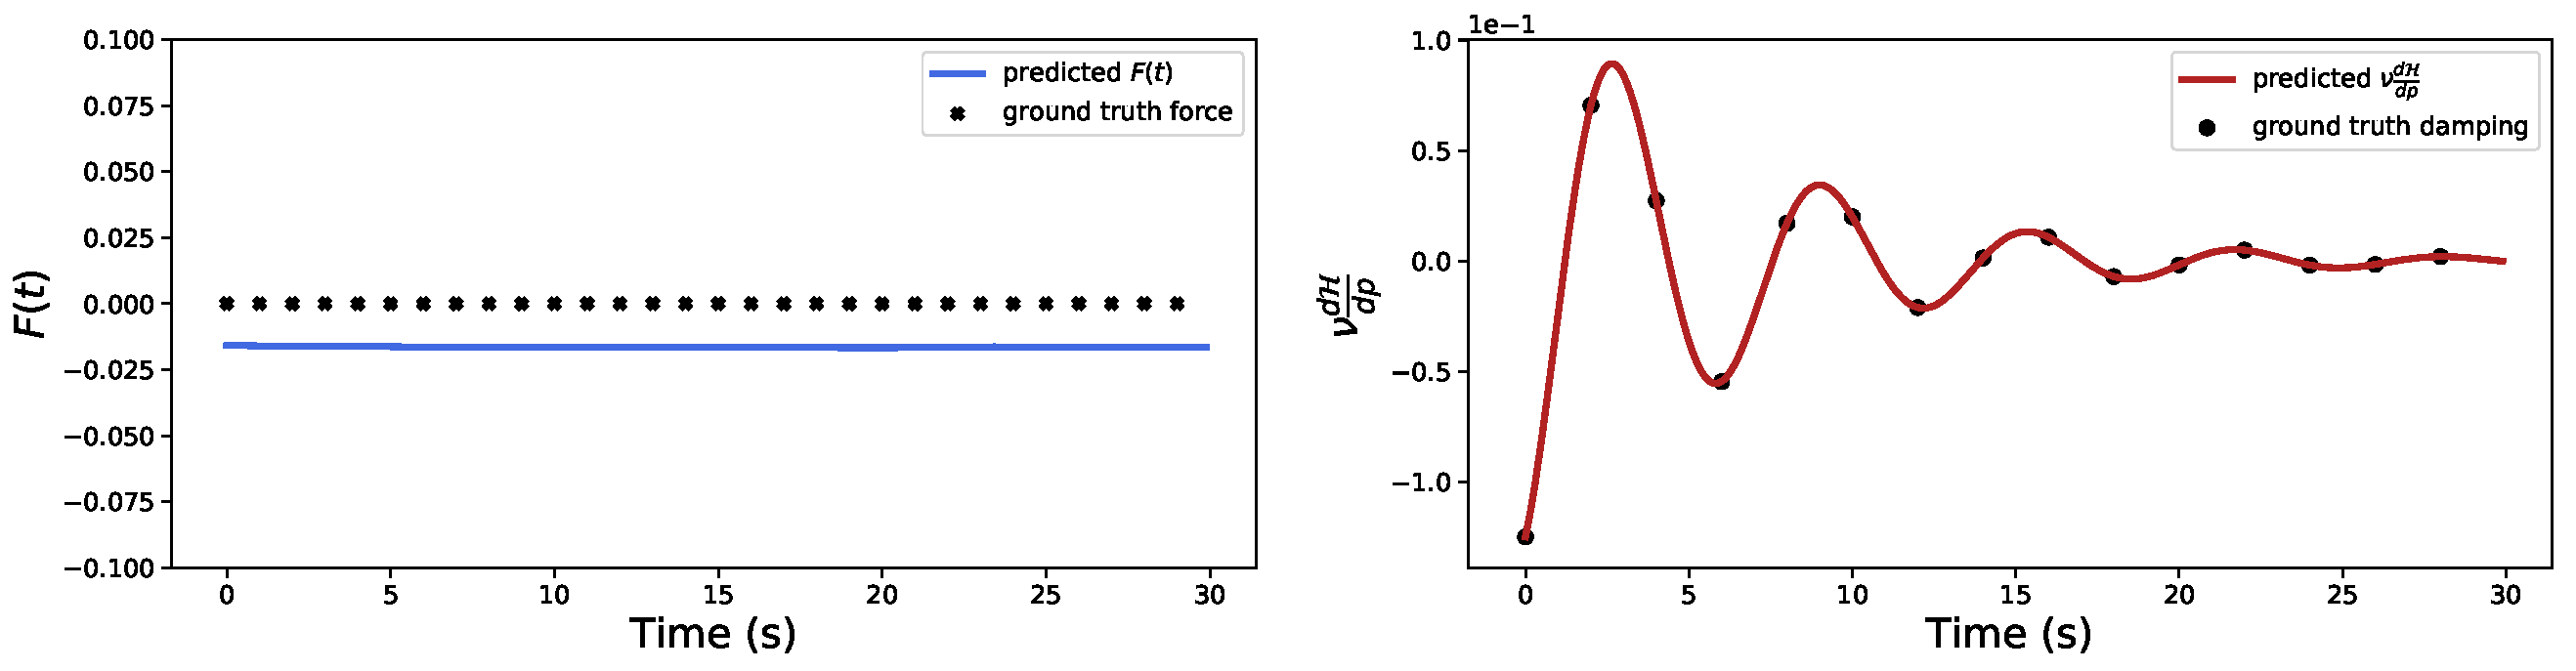
\includegraphics[width=\textwidth]{figures/figures/damped/1/damped_dpdt_new_0.pdf}
		\caption{Learnt Force and Damping terms by pHNN}
	\end{subfigure}
	\begin{subfigure}[b]{0.48\textwidth}
	    \centering
		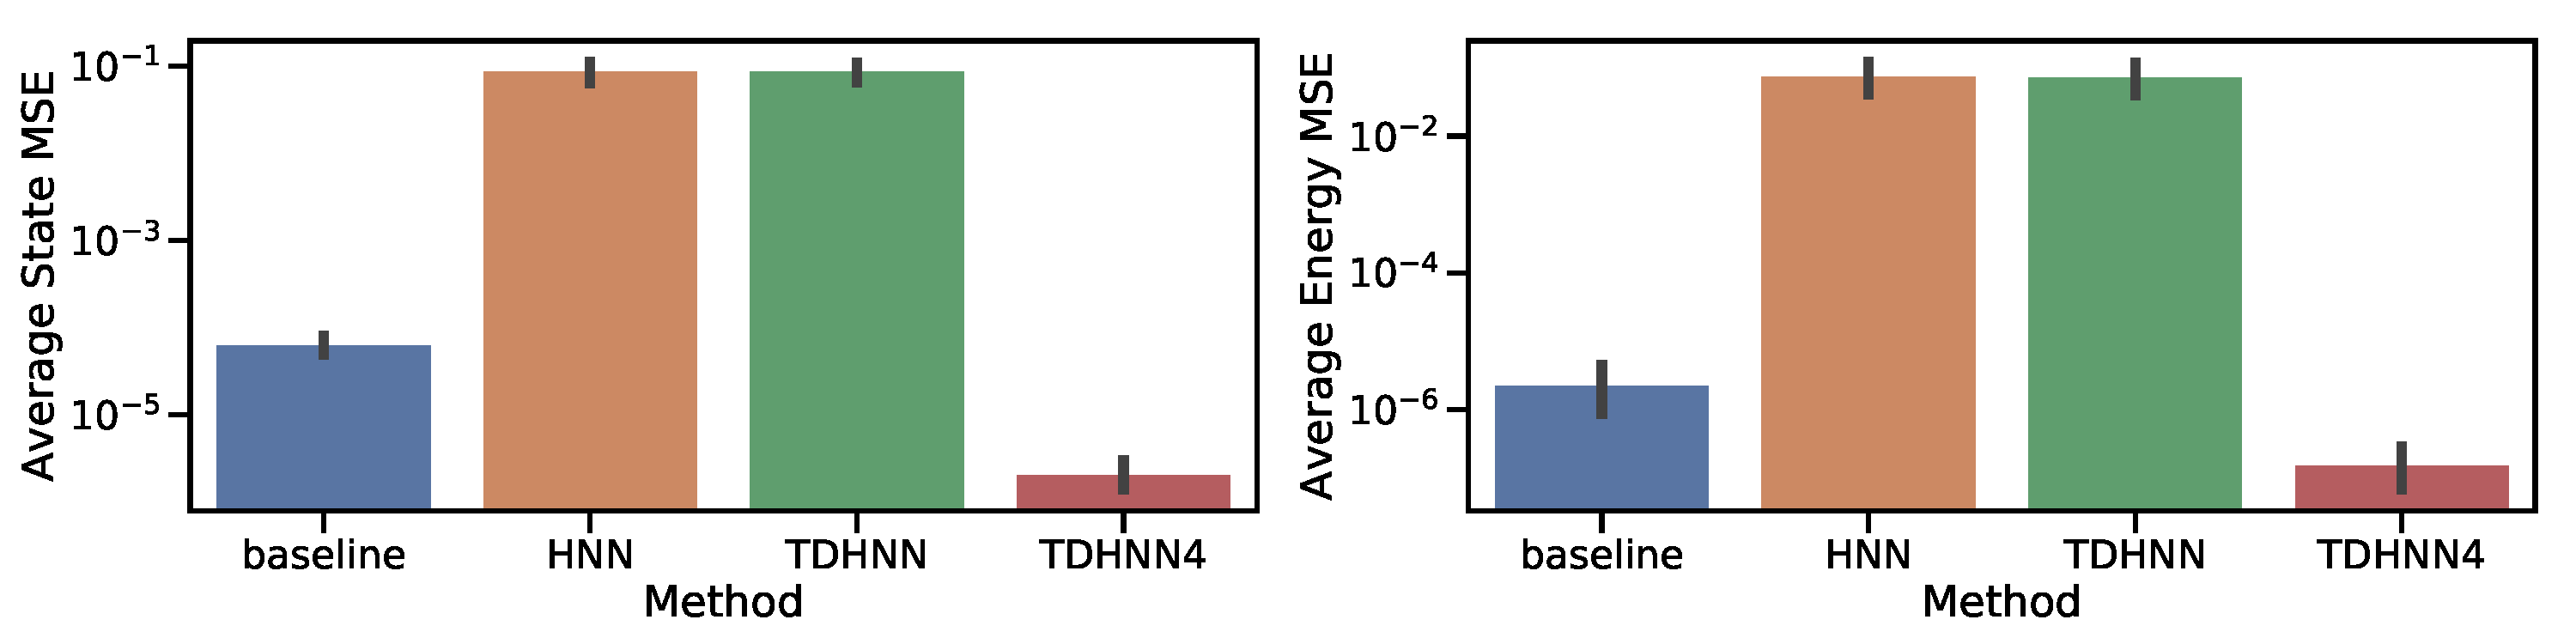
\includegraphics[width=\textwidth]{figures/figures/damped/1/damped_errors_0.pdf}
		\caption{State and energy MSE averaged across 25 initial test states}
	\end{subfigure}
\caption{Damped mass-spring setting: The baseline NN and pHNN recover the underlying dynamics well. pHNN is also able to accurately learn the damping coefficient since the predicted damping is indistinguishable from the ground truth.}
\label{damped}
\end{figure}

Firstly, we can see that both baseline NN and pHNN recover the dynamics well, whereas HNN (as expected) and TDHNN struggle to learn the damping. The main reason for this latter result is that there is no direct way of writing a scalar Hamiltonian with damping so forcing a network to do so results in unreliable test results. This result is important because it informs us that a partial inductive bias is not good at generalizing. ISecondly, we see that pHNN learns a non-zero, oscillating force. This can happen within our system because the network is not guaranteed to find the global optima and it is indeed possible for information from the Hamiltonian, $\mathcal{H}$, to leak into the force and vice-versa. This is because there is an identifiability challenge in attempting to uncover the damping and force exclusively from the state data we provide. In spite of this challenge, we find that our networks converge to reasonable forces and damping terms that can inform us of the underlying dynamics as well as help us make predictions. Thirdly, in this particular example, we do see that while the force and damping are non-zero, the force is 5 orders of magnitude smaller than $\frac{dp}{dt}$ and so its contribution is negligible.

\subsection{Forced Mass-Spring System}

Typically, while we cannot write the Hamiltonian for a damped system, we can write one for a forced system. Here, we study two types of forced mass-spring systems. The first has the following Hamiltonian form:
\begin{equation}
\mathcal{H} = \frac{1}{2}kq^2 + \frac{1}{2m}p^2 - qF_0\sin(\omega t).
\end{equation}
The second has the Hamiltonian:
\begin{equation}
\mathcal{H} = \frac{1}{2}kq^2 + \frac{1}{2m}p^2 - qF_0\sin(\omega t)\sin(2\omega t).
\end{equation}
The forced mass-spring system is typically used to study resonance and plays an important role in numerous applications including music, bridge design and molecular excitation making it an important system to investigate.

\begin{figure}[h!]
\centering
\captionsetup{justification=centering}
%	\begin{subfigure}[b]{0.4\textwidth}
%		\centering
%		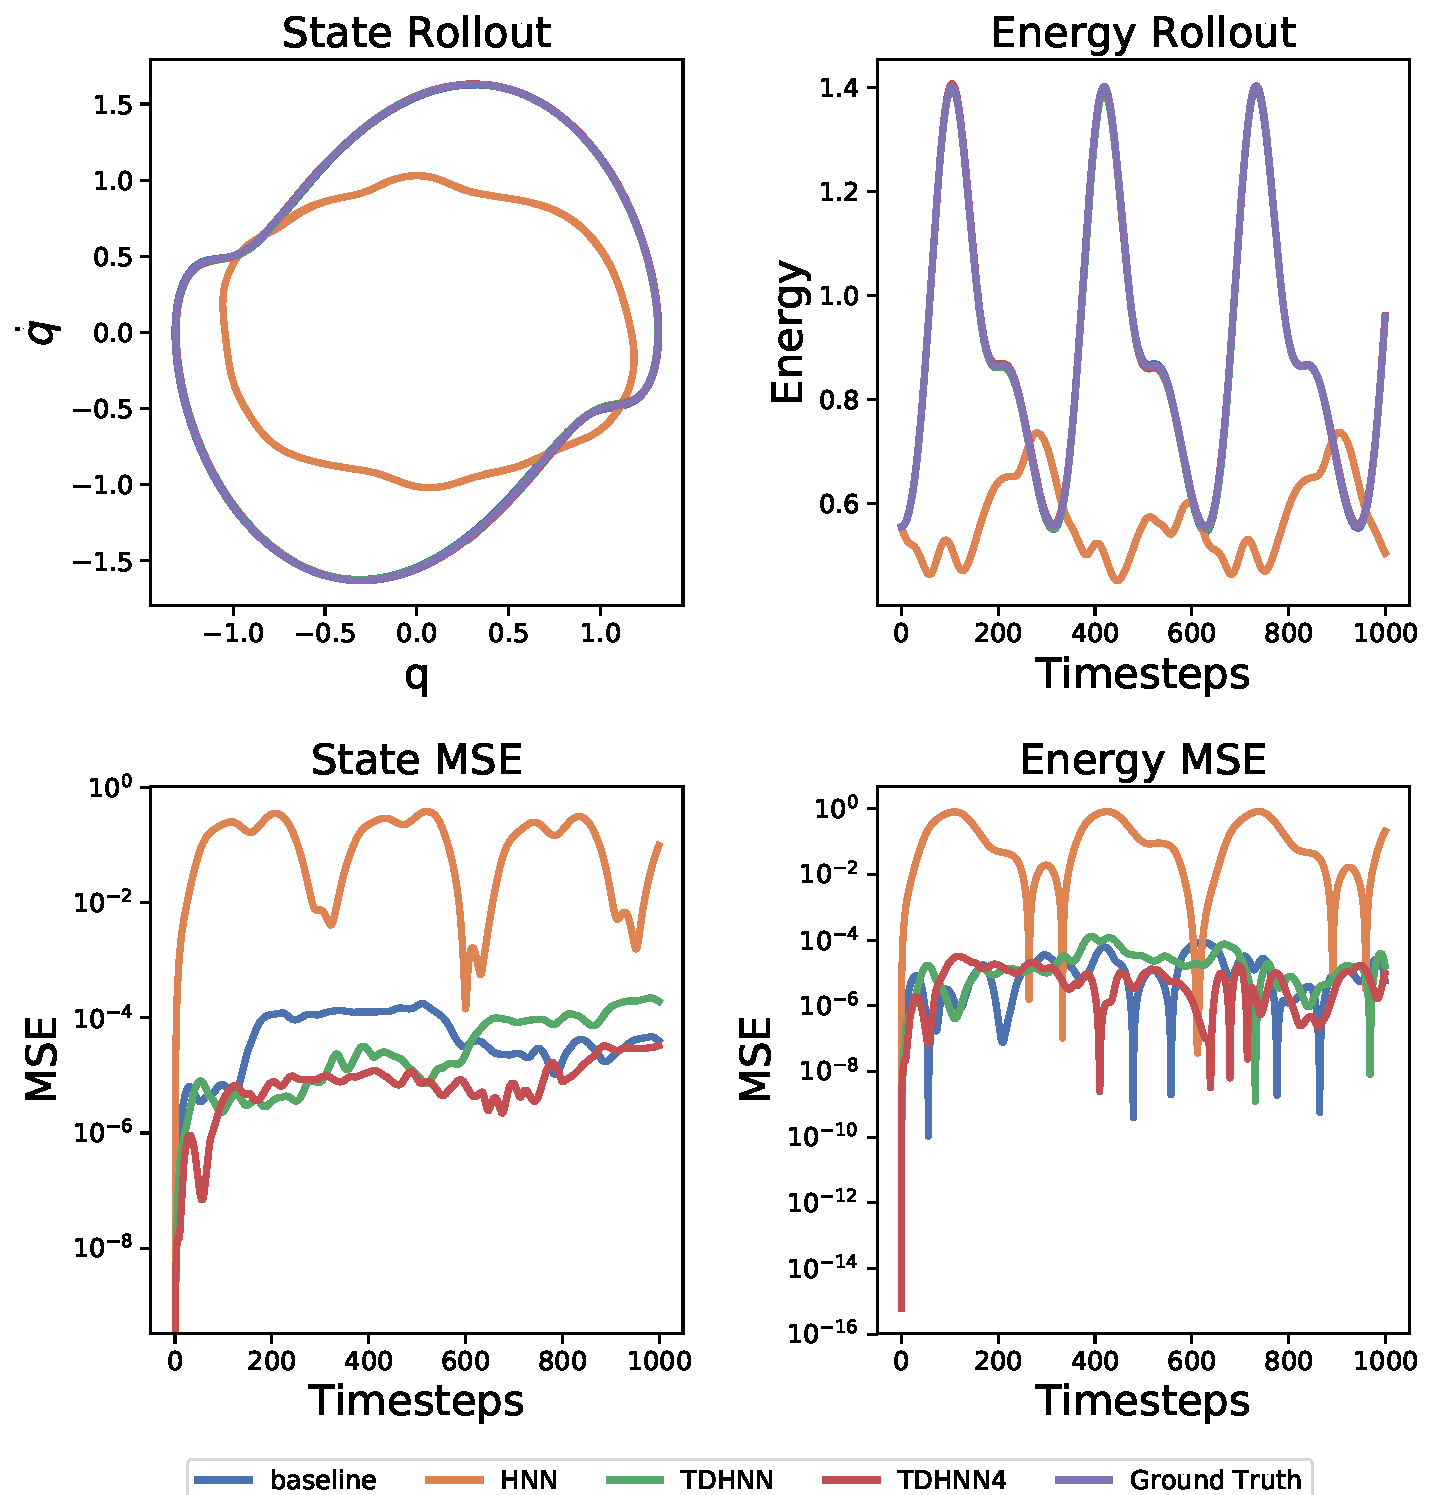
\includegraphics[width=\textwidth]{figures/forced_mass_spring_1.pdf}
%		\caption{State and energy rollout/MSE of an initial condition in the test set.}
%	\end{subfigure}
	\begin{subfigure}[b]{0.48\textwidth}
		\centering
		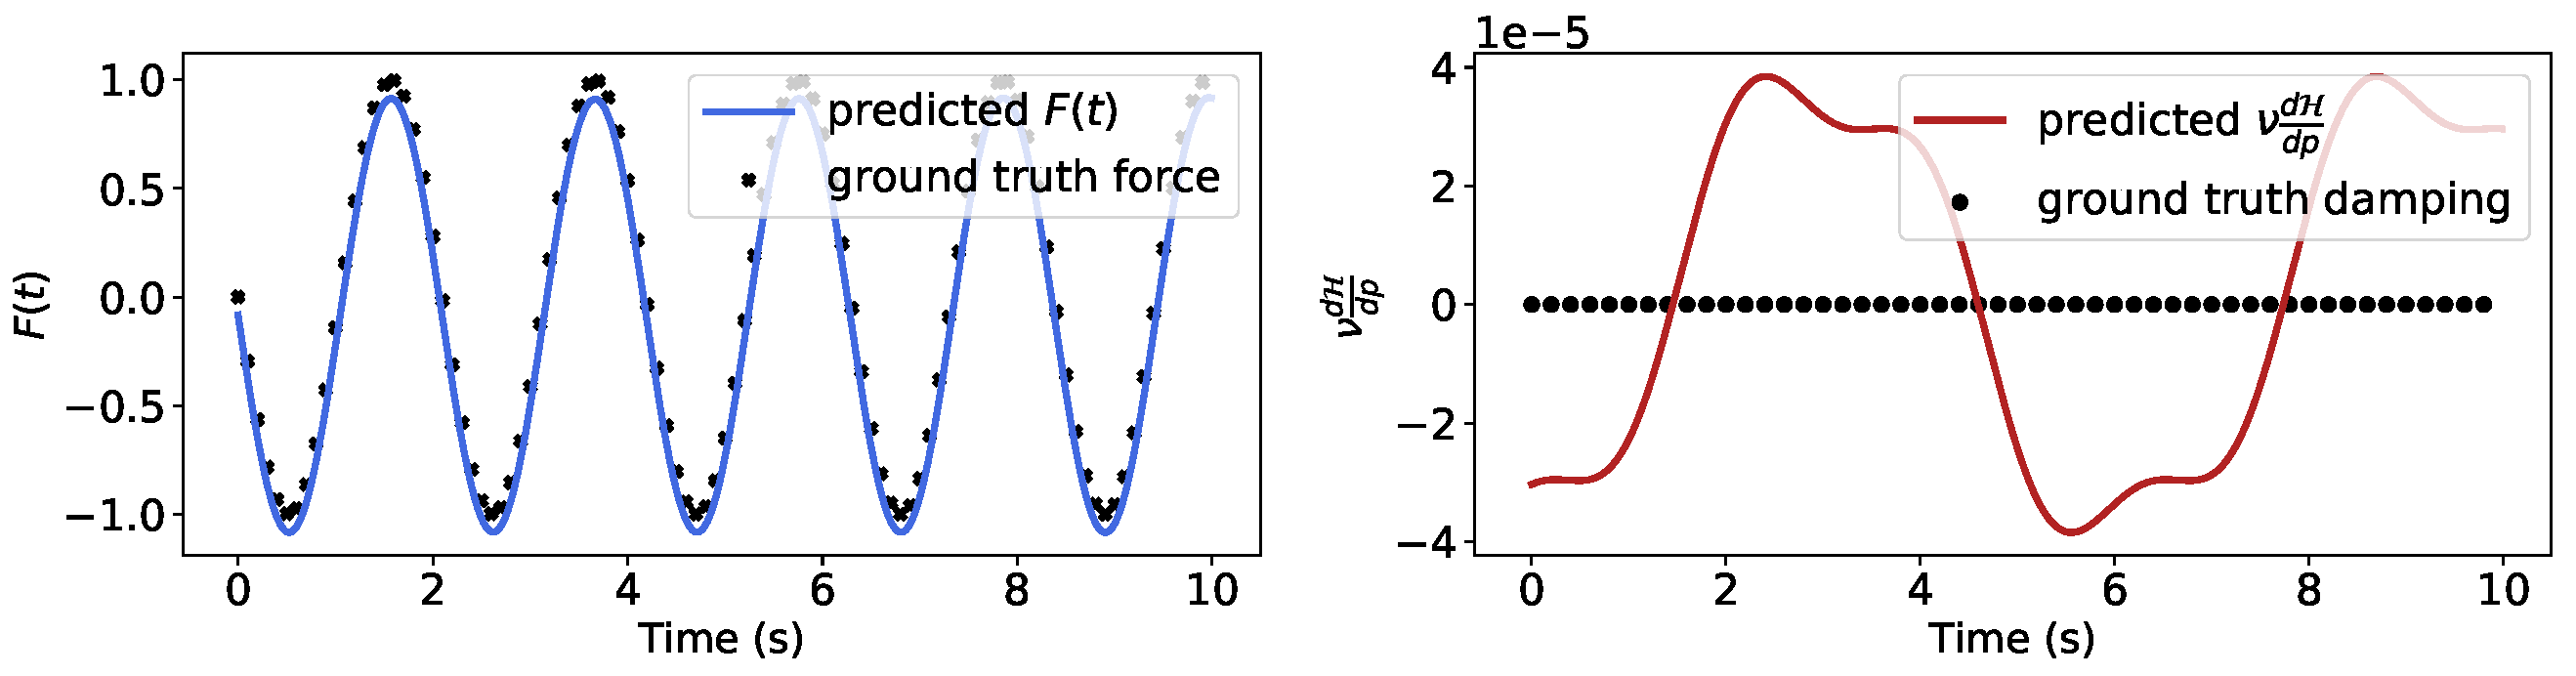
\includegraphics[width=\textwidth]{figures/figures/forced_mass_spring/1/forced_mass_spring_dpdt_new_0.pdf}
		\caption{Learnt Force and Damping terms by pHNN}
	\end{subfigure}
	\begin{subfigure}[b]{0.48\textwidth}
	    \centering
		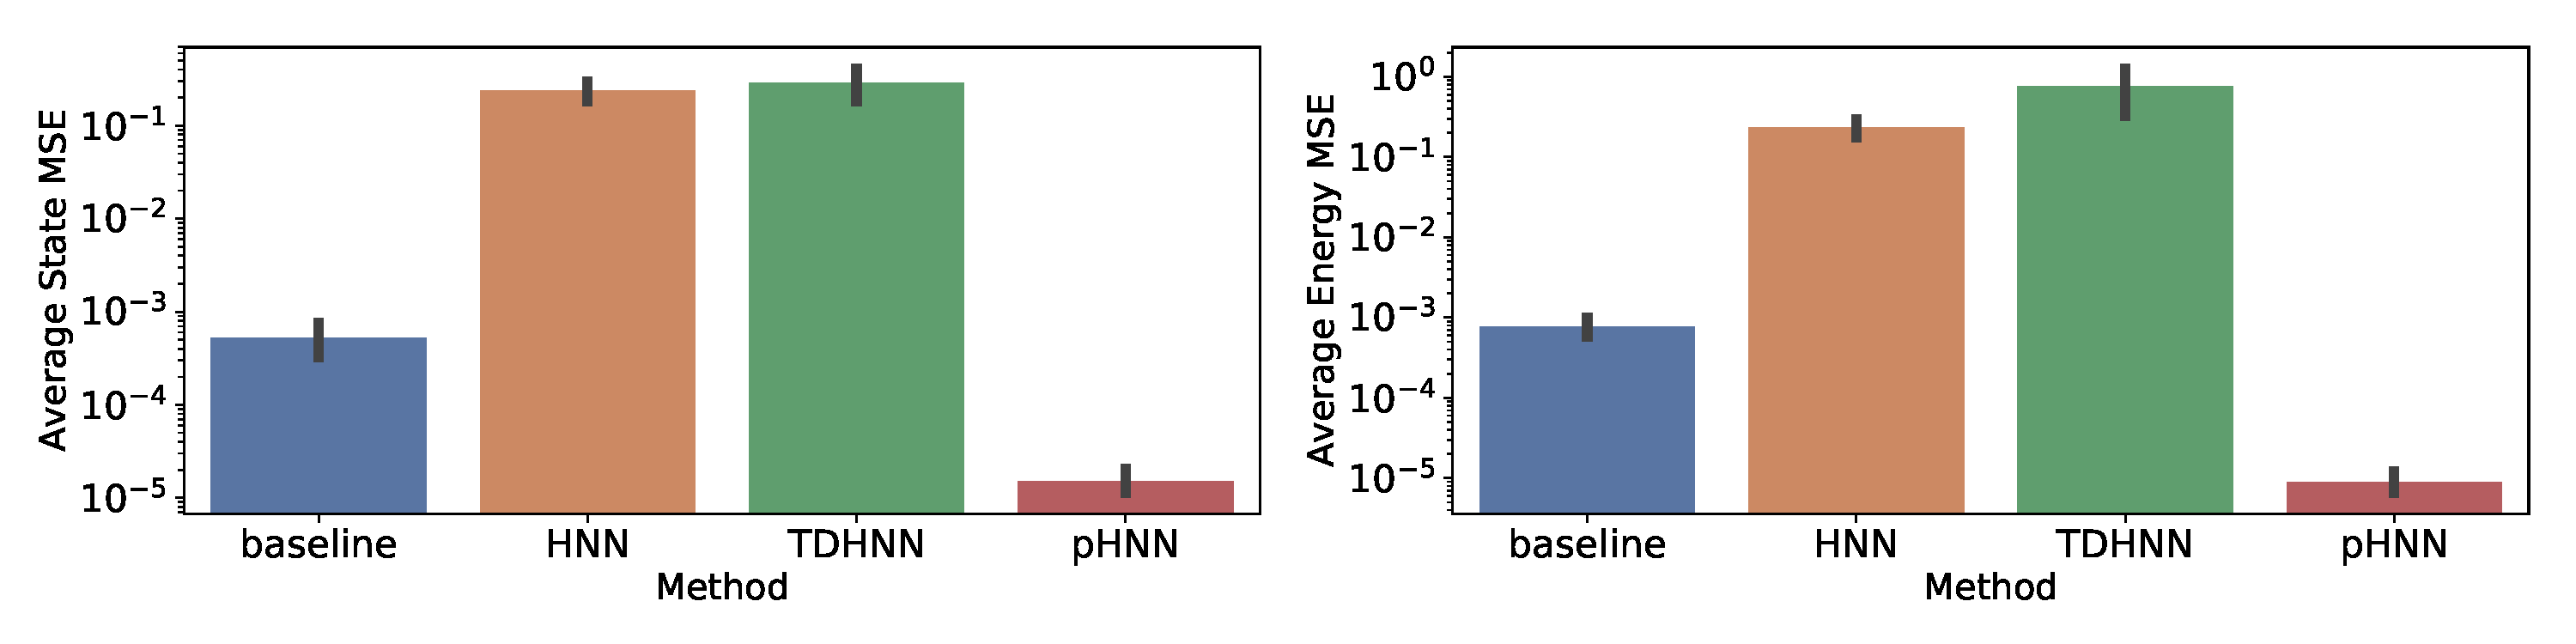
\includegraphics[width=\textwidth]{figures/figures/forced_mass_spring/1/forced_mass_spring_errors_0.pdf}
		\caption{Rollout state and energy MSE averaged across 25 initial test states}
	\end{subfigure}
\caption{Forced mass-spring (I): HNN cannot learn the underlying dynamics as it has no explicit-time dependence. pHNN shows the best performance as it explicitly learns a time-dependent force.}
\label{fig.fmspring1}
\end{figure}

\begin{figure}[h!]
\centering
\captionsetup{justification=centering}
%	\begin{subfigure}[b]{0.4\textwidth}
%		\centering
%		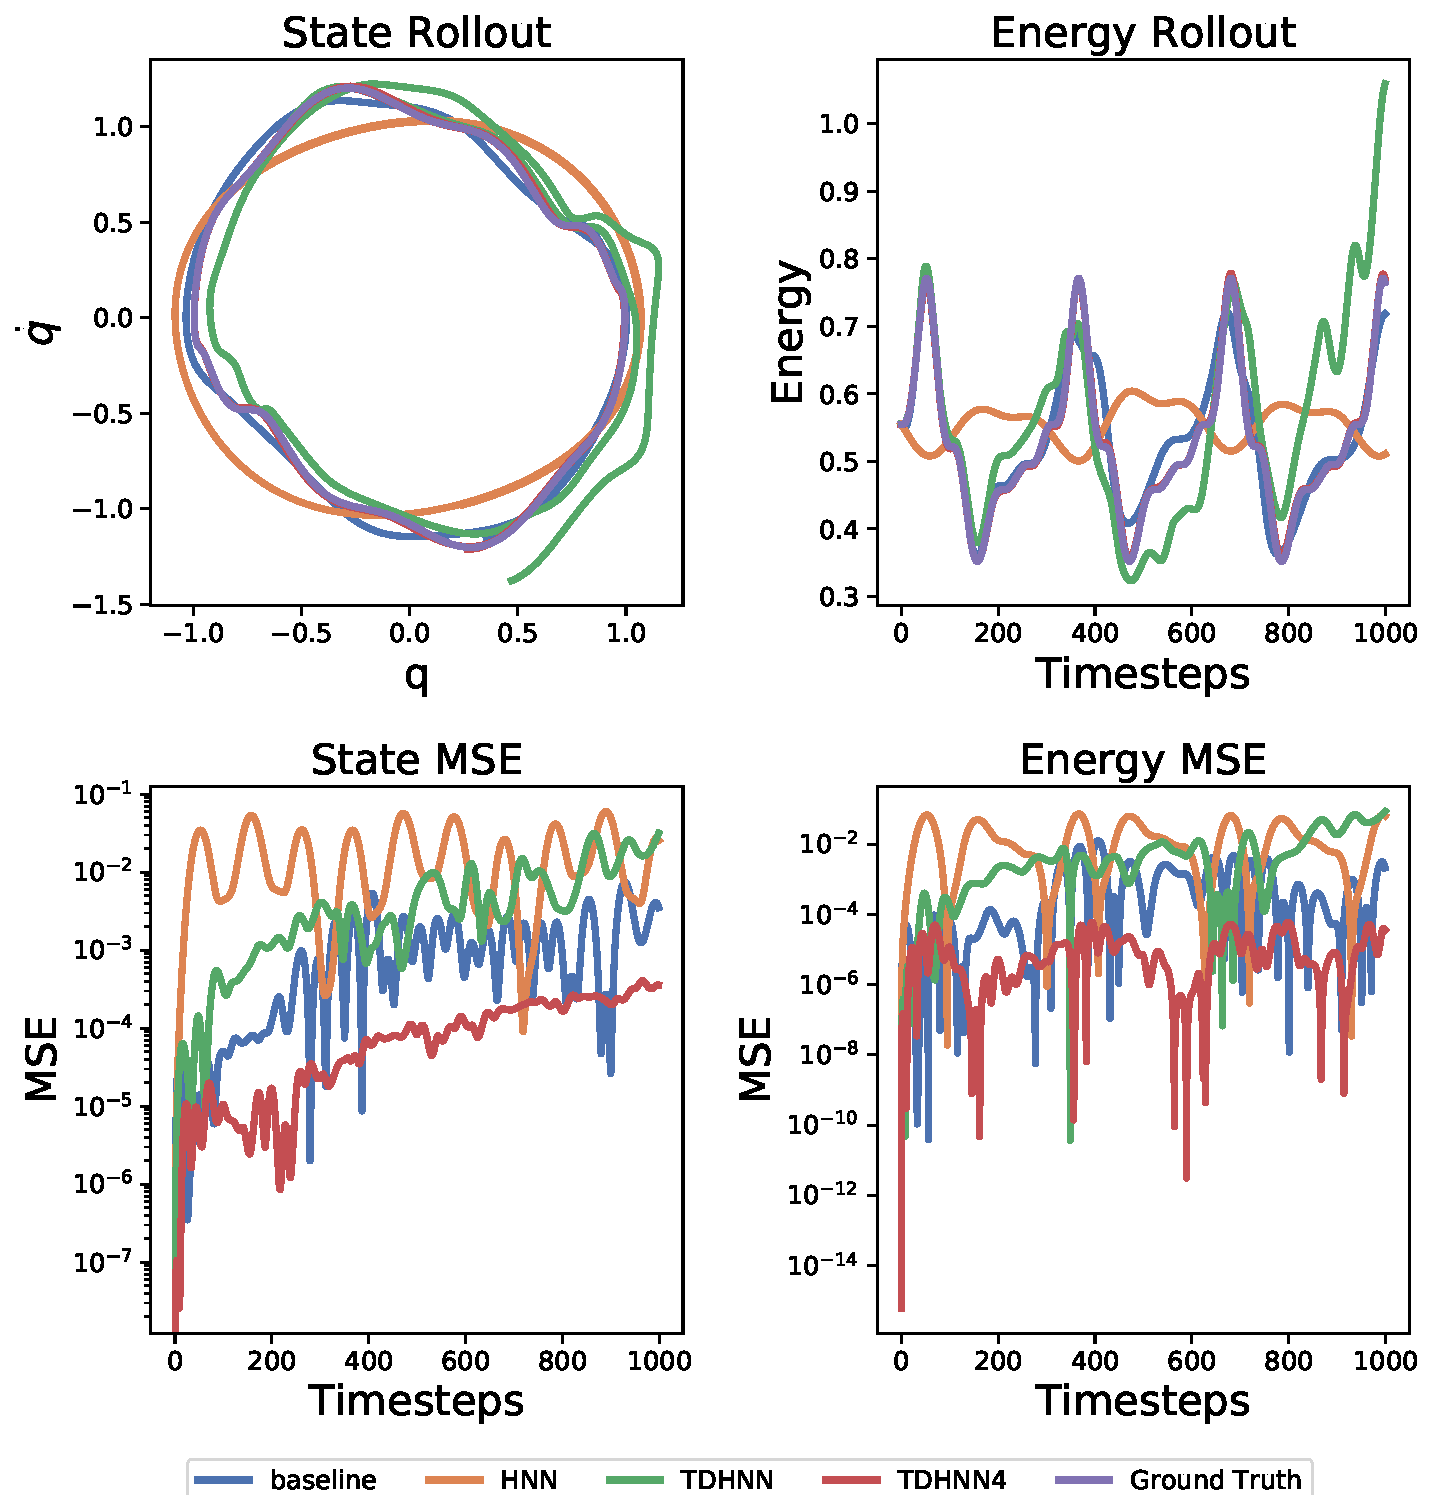
\includegraphics[width=\textwidth]{figures/forced_mass_spring_2.pdf}
%		\caption{State and energy rollout/MSE of an initial condition in the test set.}
%	\end{subfigure}
	\begin{subfigure}[b]{0.48\textwidth}
		\centering
		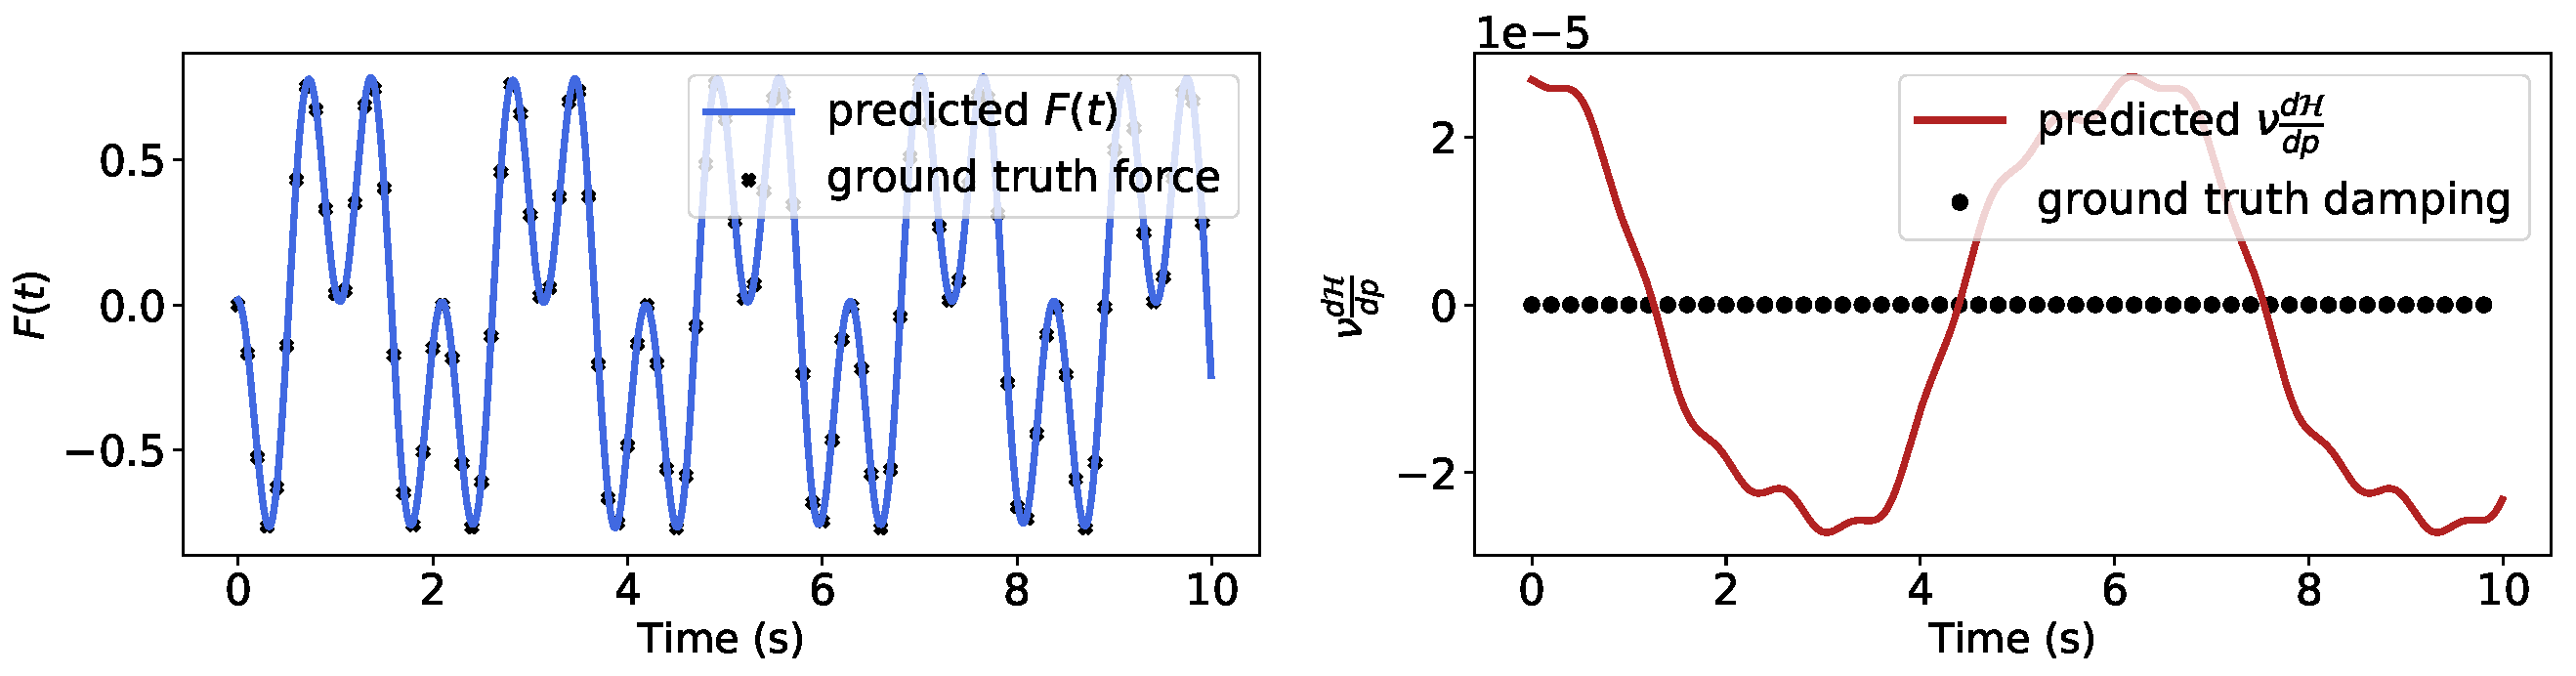
\includegraphics[width=\textwidth]{figures/figures/forced_mass_spring/2/forced_mass_spring_dpdt_new_0.pdf}
		\caption{Learnt Force and Damping terms by pHNN}
	\end{subfigure}
	\begin{subfigure}[b]{0.48\textwidth}
	    \centering
		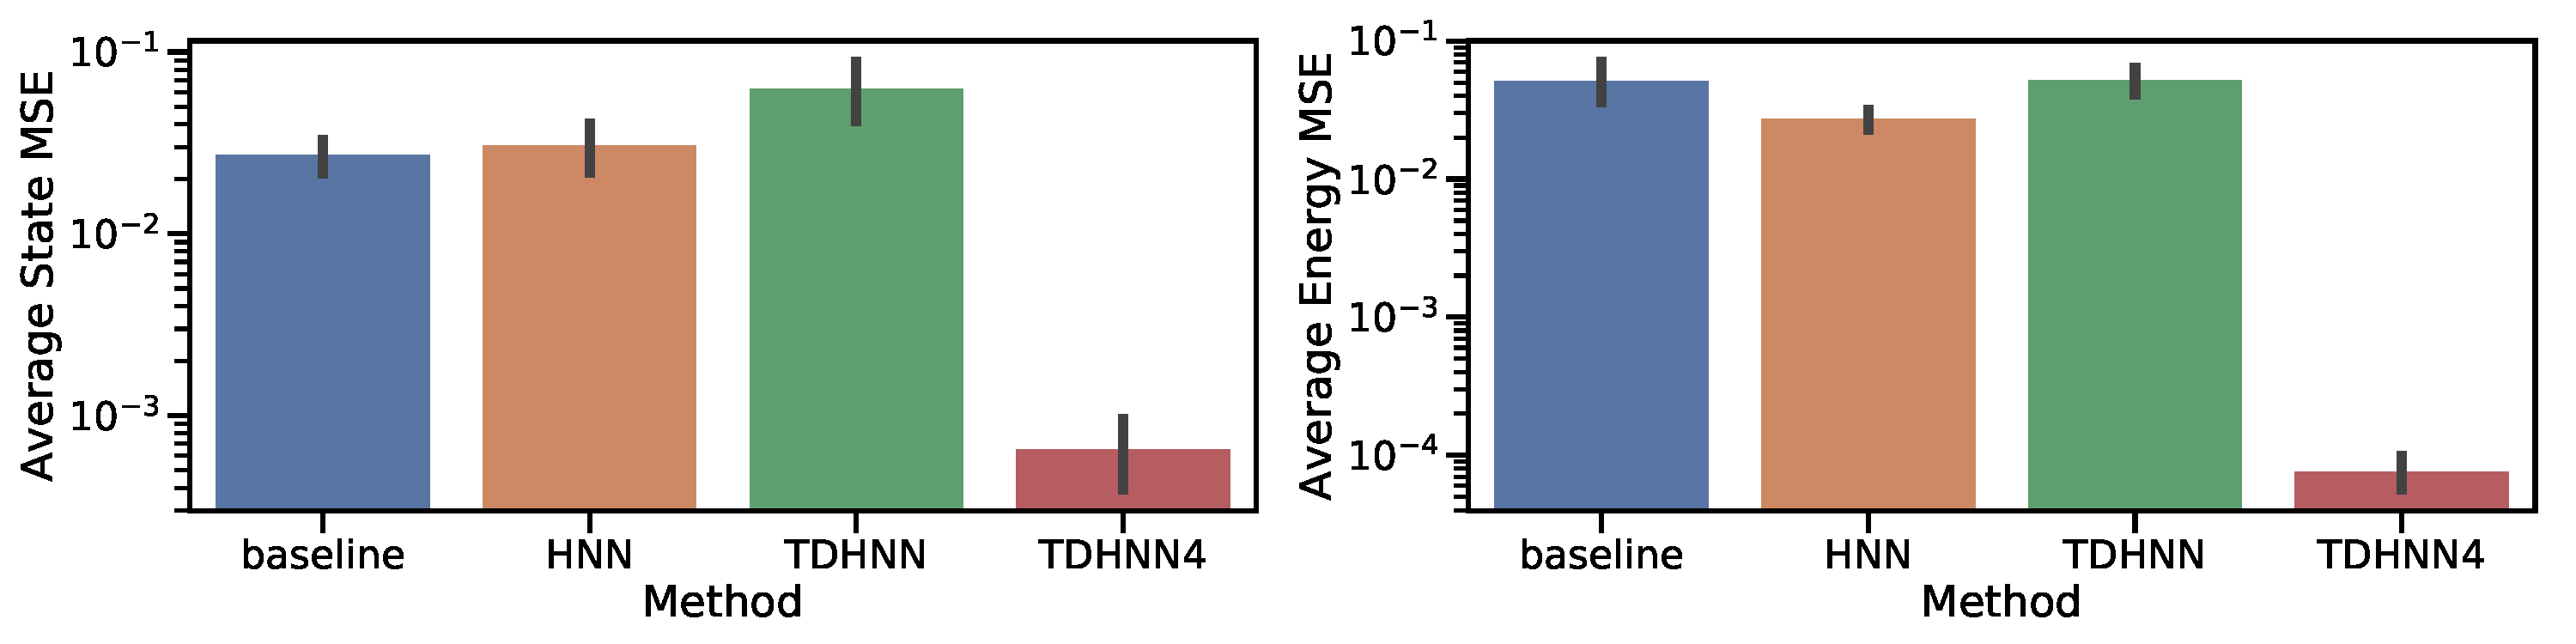
\includegraphics[width=\textwidth]{figures/figures/forced_mass_spring/2/forced_mass_spring_errors_0.pdf}
		\caption{Rollout state and energy MSE averaged across 25 initial test states}
	\end{subfigure}
\caption{Forced mass-spring (II):The time dependent force here is non-trivial, but pHNN shows it can recover it.}
\label{fig.fmspring2}
\end{figure}
\textbf{Training:} In both settings, we use 20 initial conditions, where the initial state $[q_0,p_0]$ is sampled such that $q_0^2 +p_0^2 =r_0^2$ where $1 \leq r_0 \leq 4.5$. The states are rolled out to $T_{\max}=10.01$ at a $\Delta t = 0.01$. $k$, $m$ and $F_0$ are all set to 1 without loss of generality. The forcing frequency $\omega$ is set to 3. 

\textbf{Test:} At inference, we compute the rollout of 25 unseen initial conditions, and report the average state and energy rollout MSE in the Fig. \ref{fig.fmspring1} and Fig. \ref{fig.fmspring2}.

We study both systems here to illustrate that while the baseline NN is able to do relatively well in comparison to pHNN with a simple force, a more complex force significantly hurts its performance in terms of state/energy MSE. More importantly, we see that for both systems pHNN can recover the ground truth force quite precisely and while they both learn a non-zero damping term, their contribution to $\frac{dp}{dt}$ is negligible. 

\subsection{Duffing Equation}

We now investigate the Duffing equation that brings both forcing and damping to the mass-spring system. We do note that the unforced and undamped regular Hamiltonian $\mathcal{H}_{reg}$ of the Duffing system is:
\begin{equation}
\mathcal{H}_{reg} = \frac{p^2}{2m}+ \alpha \frac{q^2}{2} + \beta \frac{q^4}{4}.
\end{equation}
Unlike the simple mass-spring system, the Duffing equation has an additional quartic function of $q$. This means that the shape of the potential function can be a double-well or a single well based on the coefficients $\alpha$ and $\beta$. The general Duffing equation combines both the force and damping terms discussed previously with $\frac{d\mathcal{H}_{reg}}{dq}$. Typically the equation is written as:
\begin{equation}
\ddot{q} = -\delta \dot{q} -\alpha q -\beta q^3 +\gamma \sin(\omega t). 
\end{equation}
A combination of parameters $\alpha,\beta,\delta,\gamma,\omega$ will make the Duffing system either chaotic or non-chaotic. We study both regimes.

\begin{figure}[h!]
\centering
\captionsetup{justification=centering}
%	\begin{subfigure}[b]{0.4\textwidth}
%		\centering
%		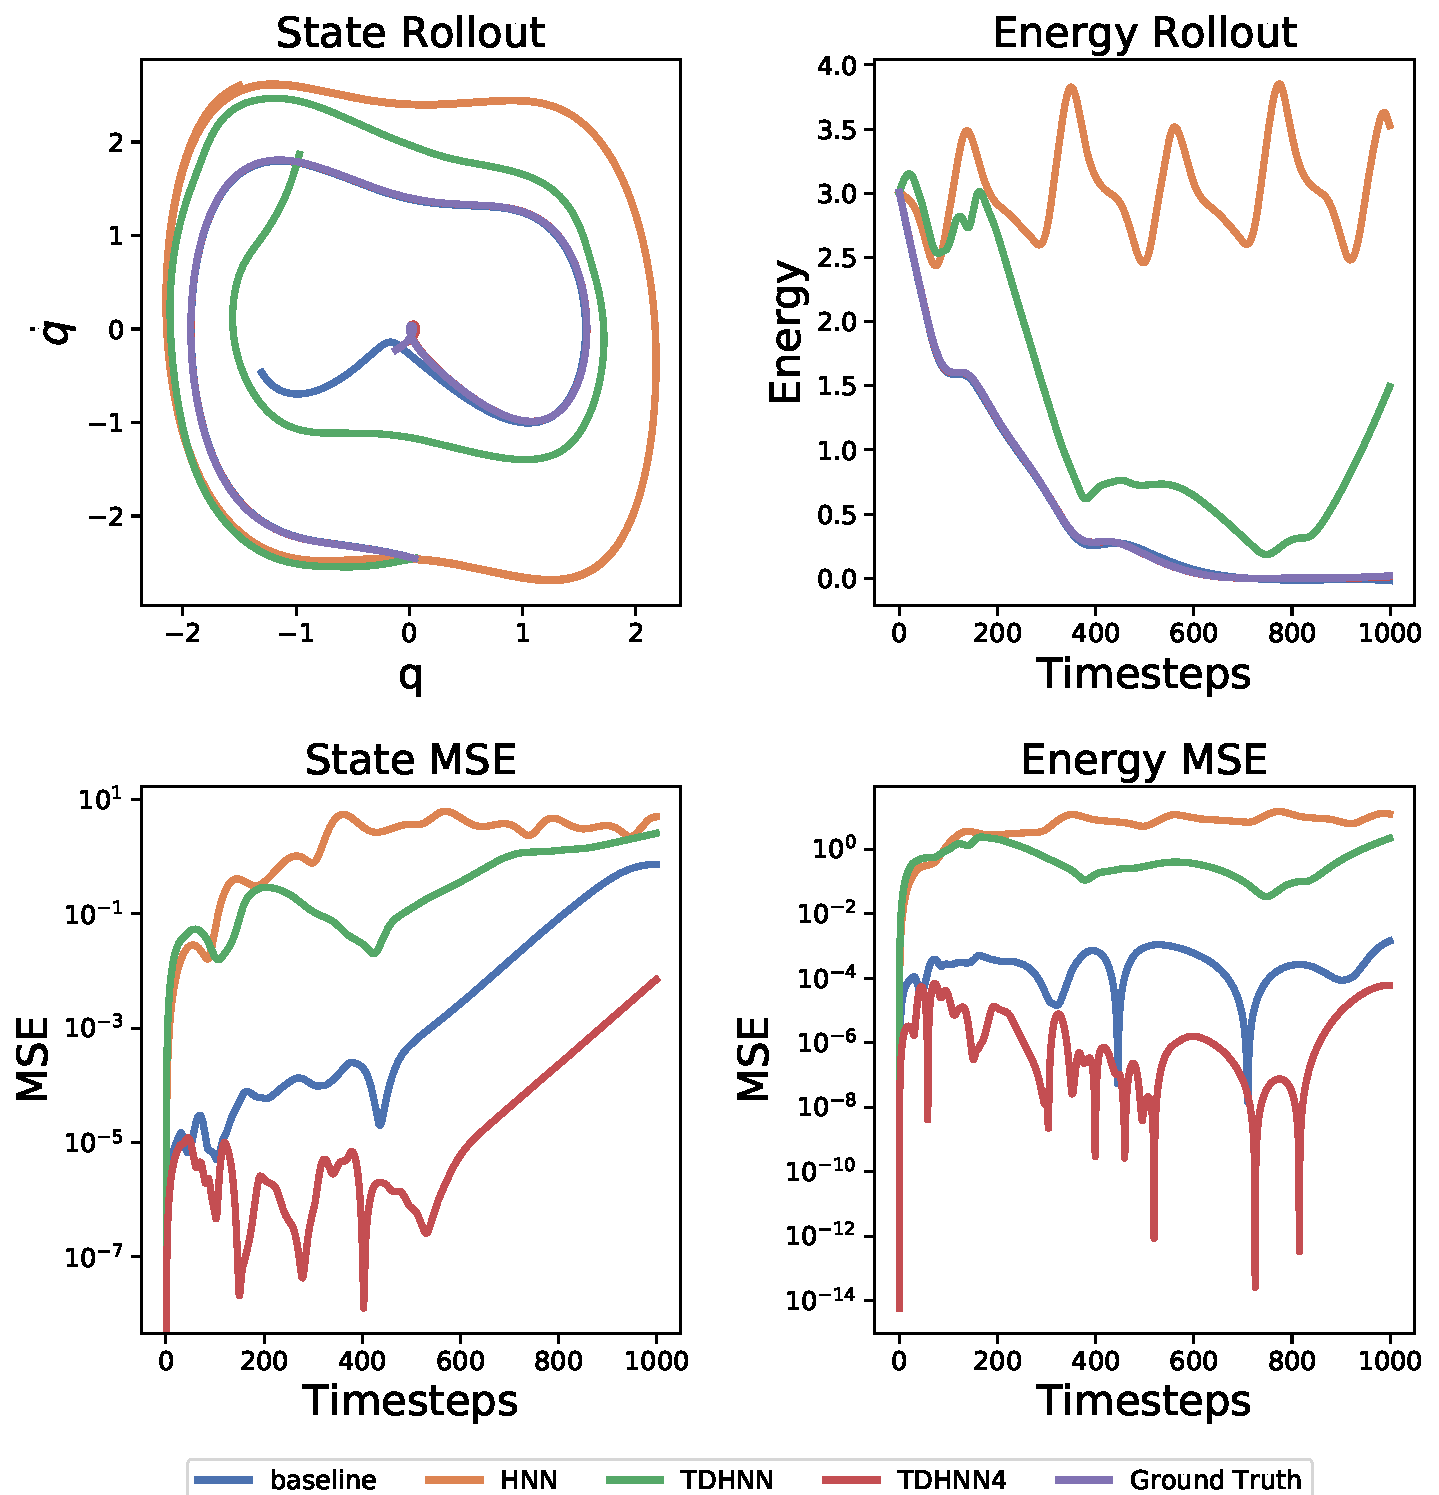
\includegraphics[width=\textwidth]{figures/duffing_state.pdf}
%		\caption{State and energy rollout/MSE of an initial condition in the test set.}
%	\end{subfigure}
	\begin{subfigure}[b]{0.48\textwidth}
		\centering
		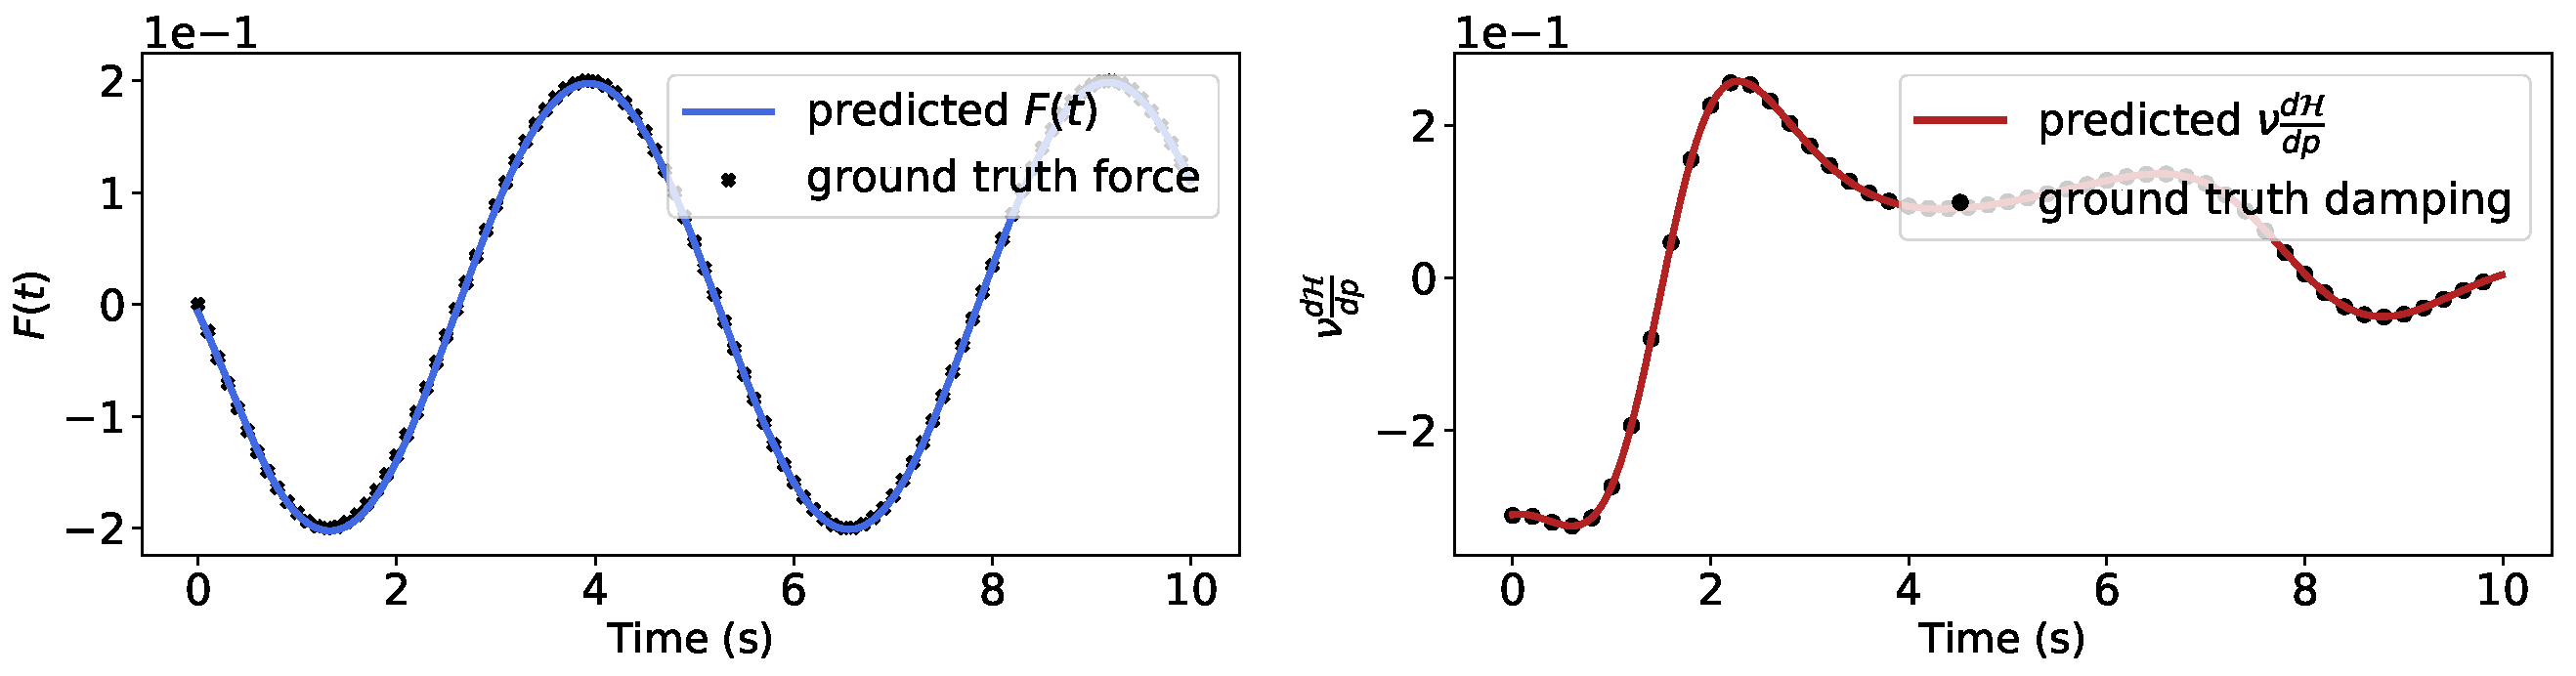
\includegraphics[width=\textwidth]{figures/figures/duffing/1/duffing_dpdt_new_0.pdf}
		\caption{Learnt Force and Damping terms of pHNN}
	\end{subfigure}
	\begin{subfigure}[b]{0.48\textwidth}
	    \centering
		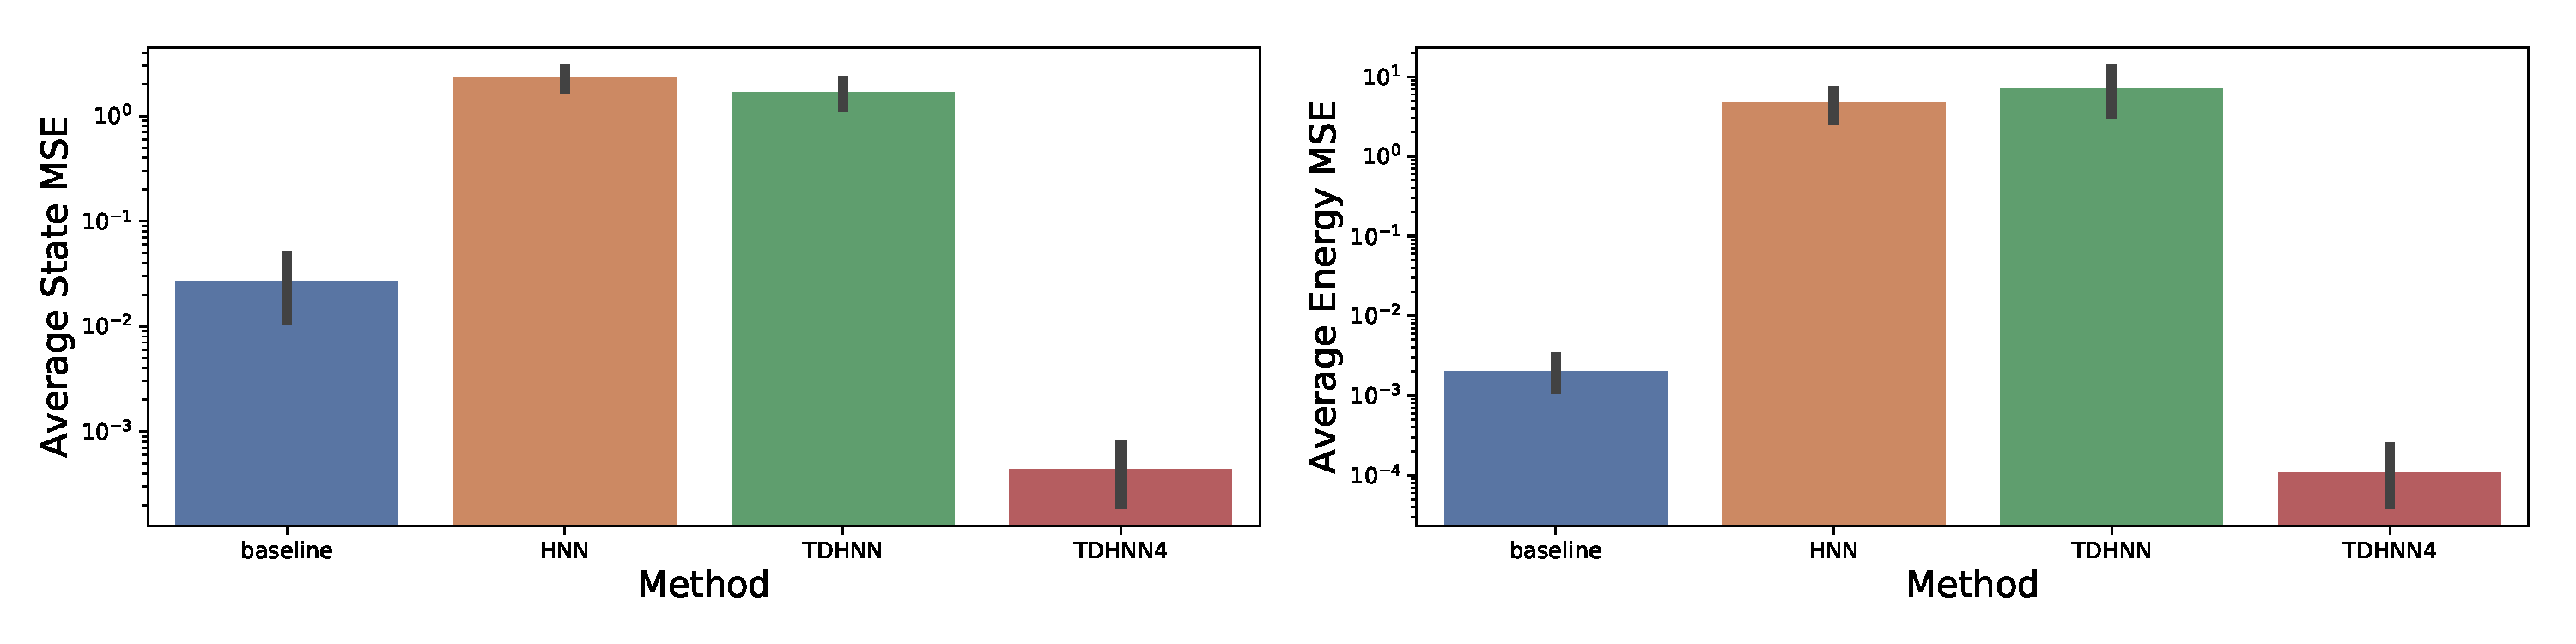
\includegraphics[width=\textwidth]{figures/figures/duffing/1/duffing_errors_0.pdf}
		\caption{State and energy MSE averaged across 25 initial test states}
	\end{subfigure}
\caption{Duffing equation (non-chaotic): pHNN significantly outperforms the other methods and is able to extract the ground truth force and damping coefficient.}
\label{fig.duffing}
\end{figure}

\begin{figure}[h!]
\centering
\captionsetup{justification=centering}
%	\begin{subfigure}[b]{0.4\textwidth}
%		\centering
%		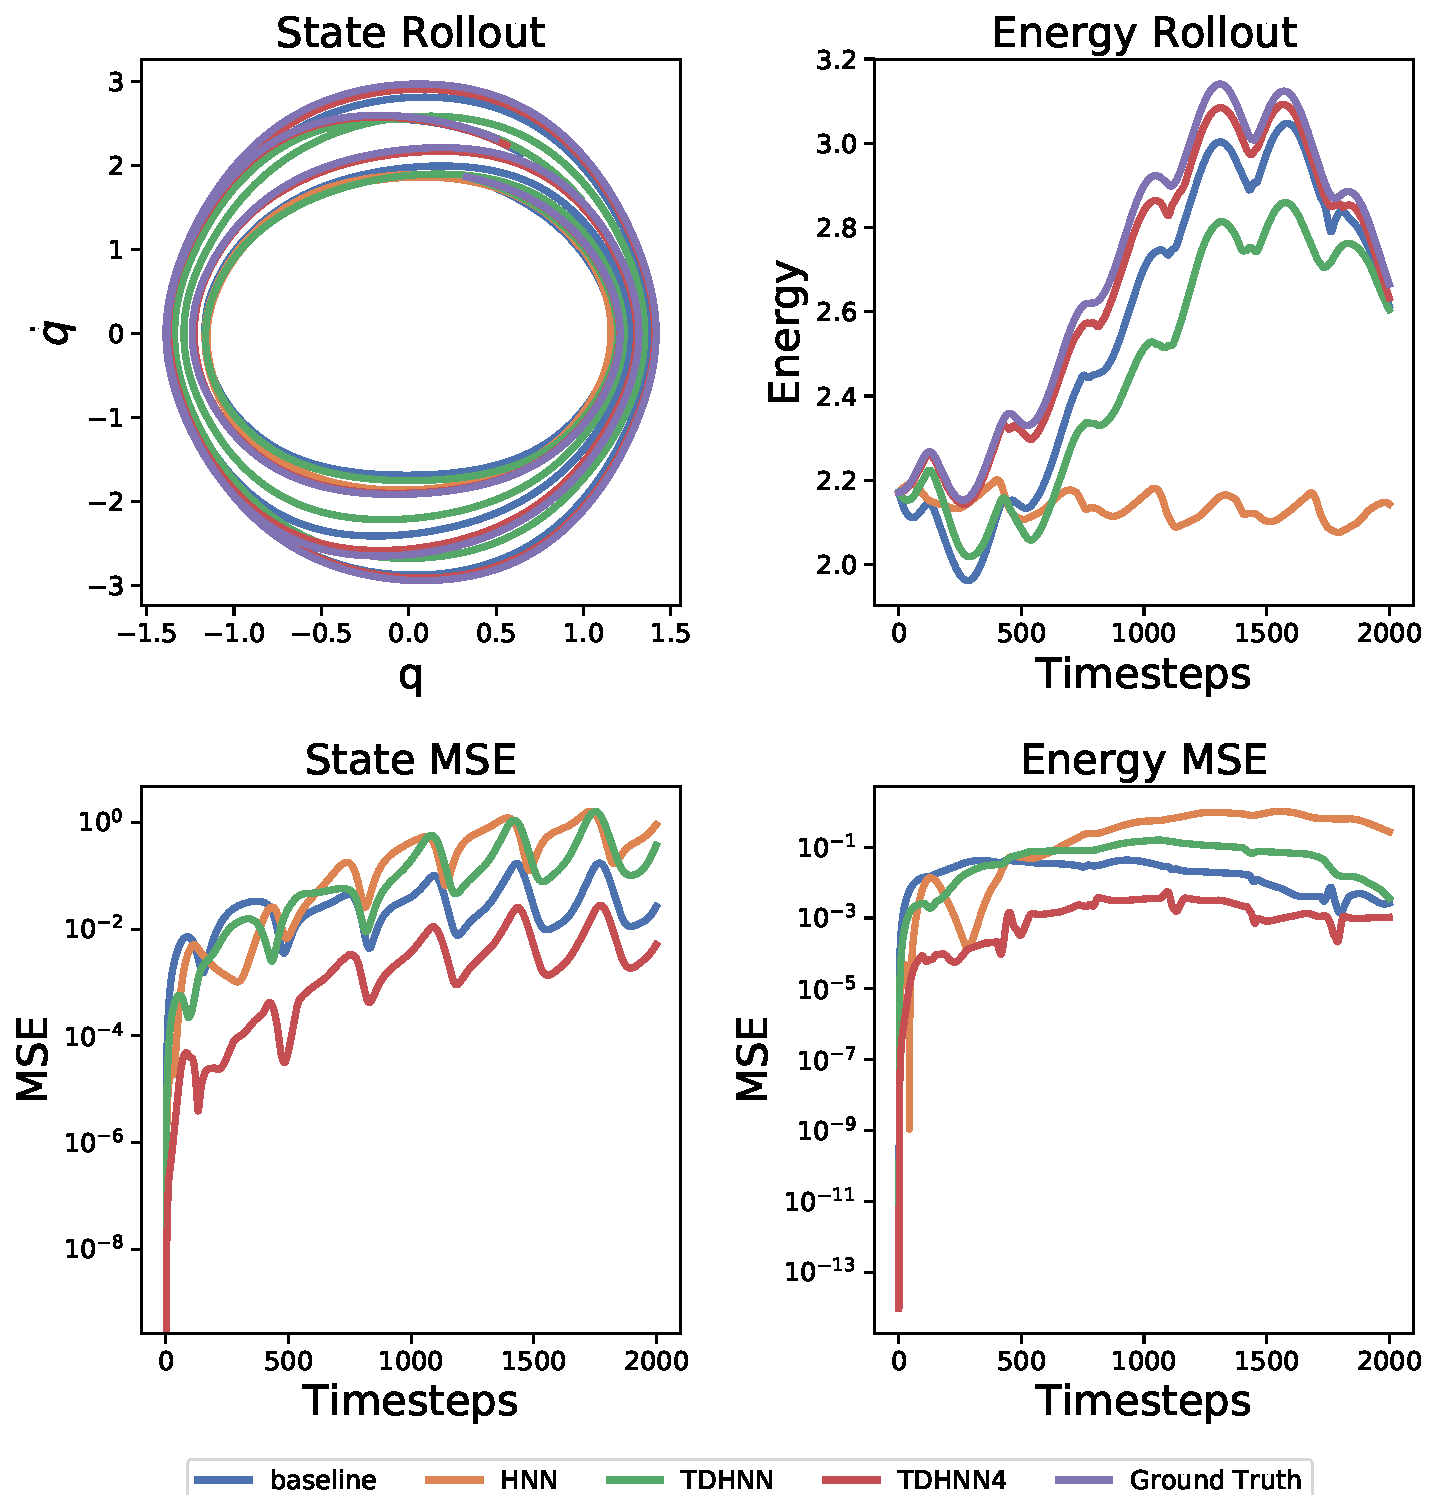
\includegraphics[width=\textwidth]{figures/relativity_pred.pdf}
%		\caption{State and energy rollout/MSE of an initial condition in the test set.}
%	\end{subfigure}
	\begin{subfigure}[b]{0.48\textwidth}
		\centering
		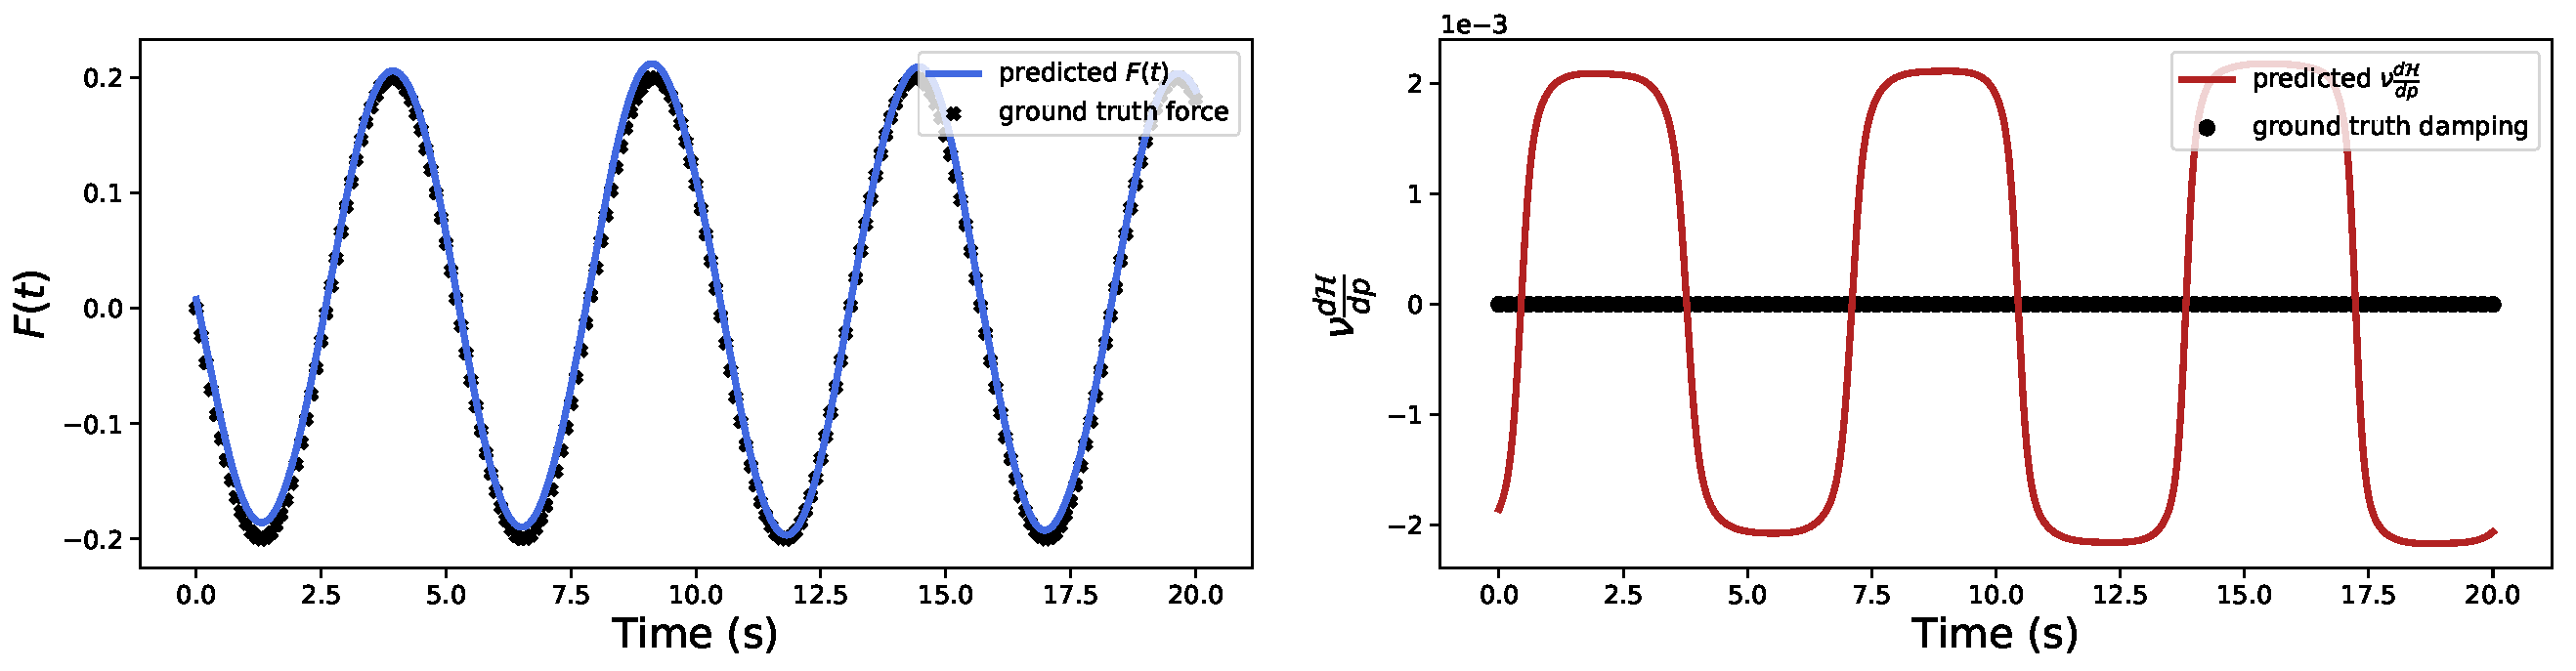
\includegraphics[width=\textwidth]{figures/figures/relativity/1/relativity_dpdt_new_0.pdf}
		\caption{Learnt Force and Damping terms of pHNN}
	\end{subfigure}
	\begin{subfigure}[b]{0.48\textwidth}
	    \centering
		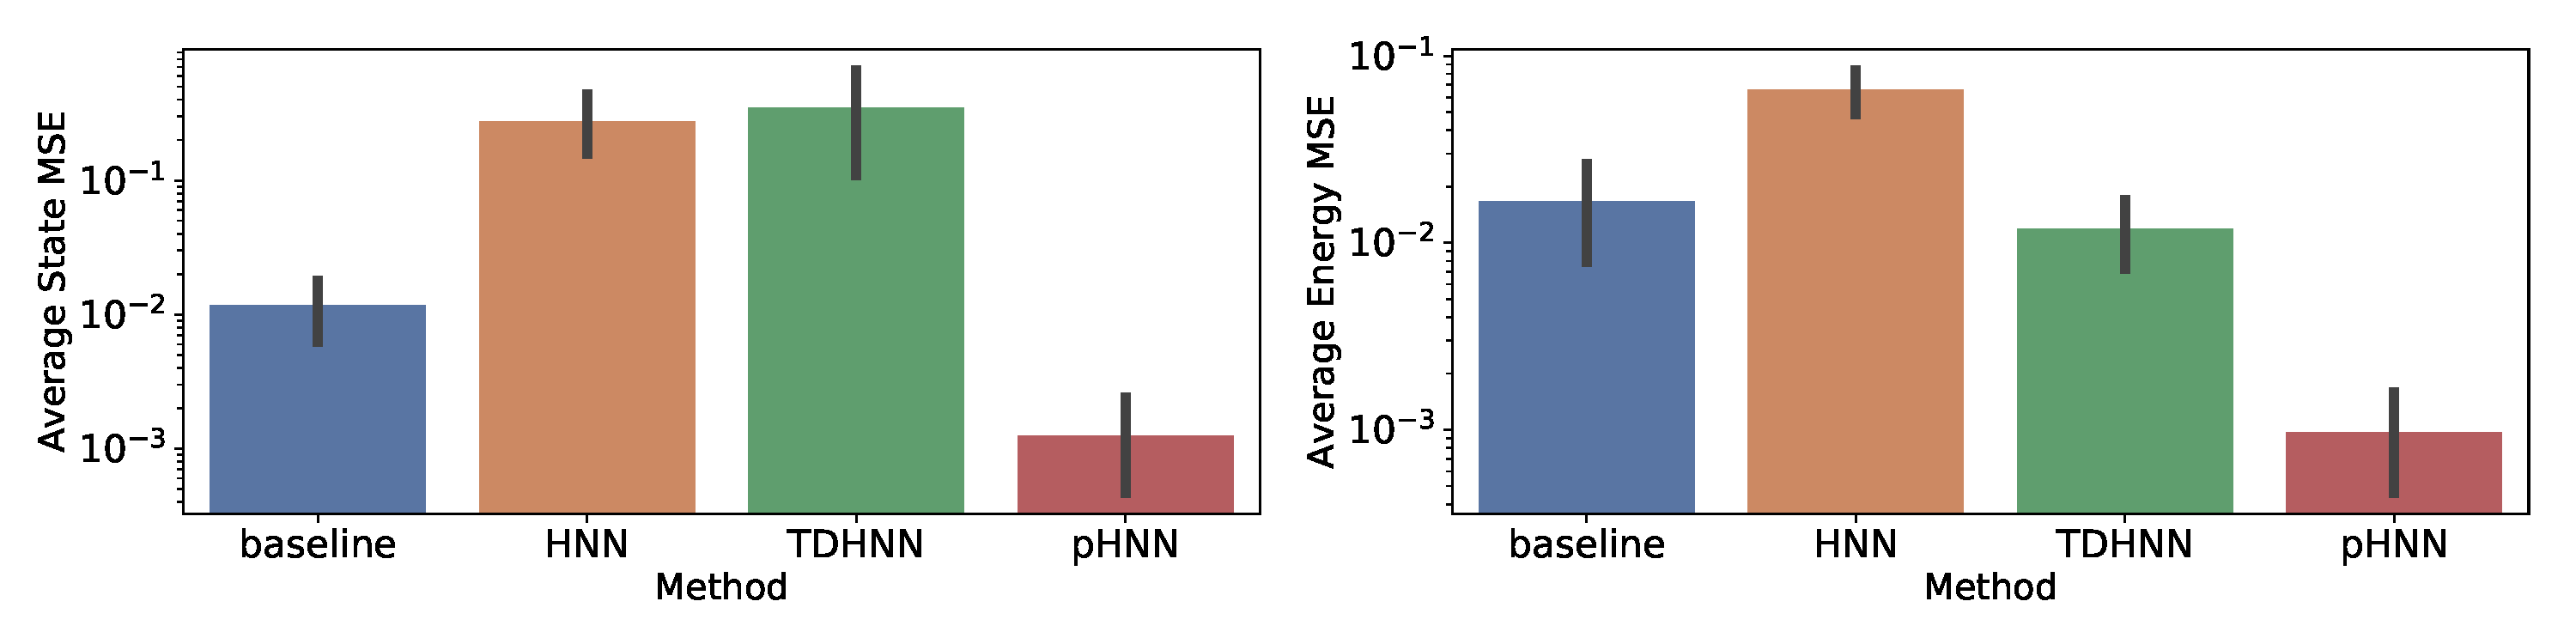
\includegraphics[width=\textwidth]{figures/figures/relativity/1/relativity_errors_0.pdf}
		\caption{Rollout state and energy MSE averaged across 25 initial test states}
	\end{subfigure}
\caption{Learned dynamics of a relativistic Duffing system.}
\end{figure}
\subsubsection{Non-Chaotic Regime}

Given a set of initial parameters for the Duffing equation: $\alpha =-1,\beta=1,\delta=0.3,\gamma=0.2,\omega=1.2$ we can obtain training data for the non-chaotic regime of the Duffing equation. 

\textbf{Training:} We uniformly sample initial conditions in $[-1,1]^2$. We use 25 initial conditions for training, rolled out to $T_{\max}=10.01$ and $\Delta t =0.01$ for the non-chaotic regime. 

\textbf{Test:} We integrate 25 unseen initial conditions at inference using the same conditions as above and evaluate both energy and state MSE (see Fig.\ref{fig.duffing}).

In addition to learning the force and damping terms accurately, inspecting the predicted Hamiltonian over a 2-D grid of position and momentum values shows that pHNN can also accurately learn the functional form of $\mathcal{H}_{reg}$ (see Fig.\ref{duffing_ham}).

\begin{figure*}[h]
\centering
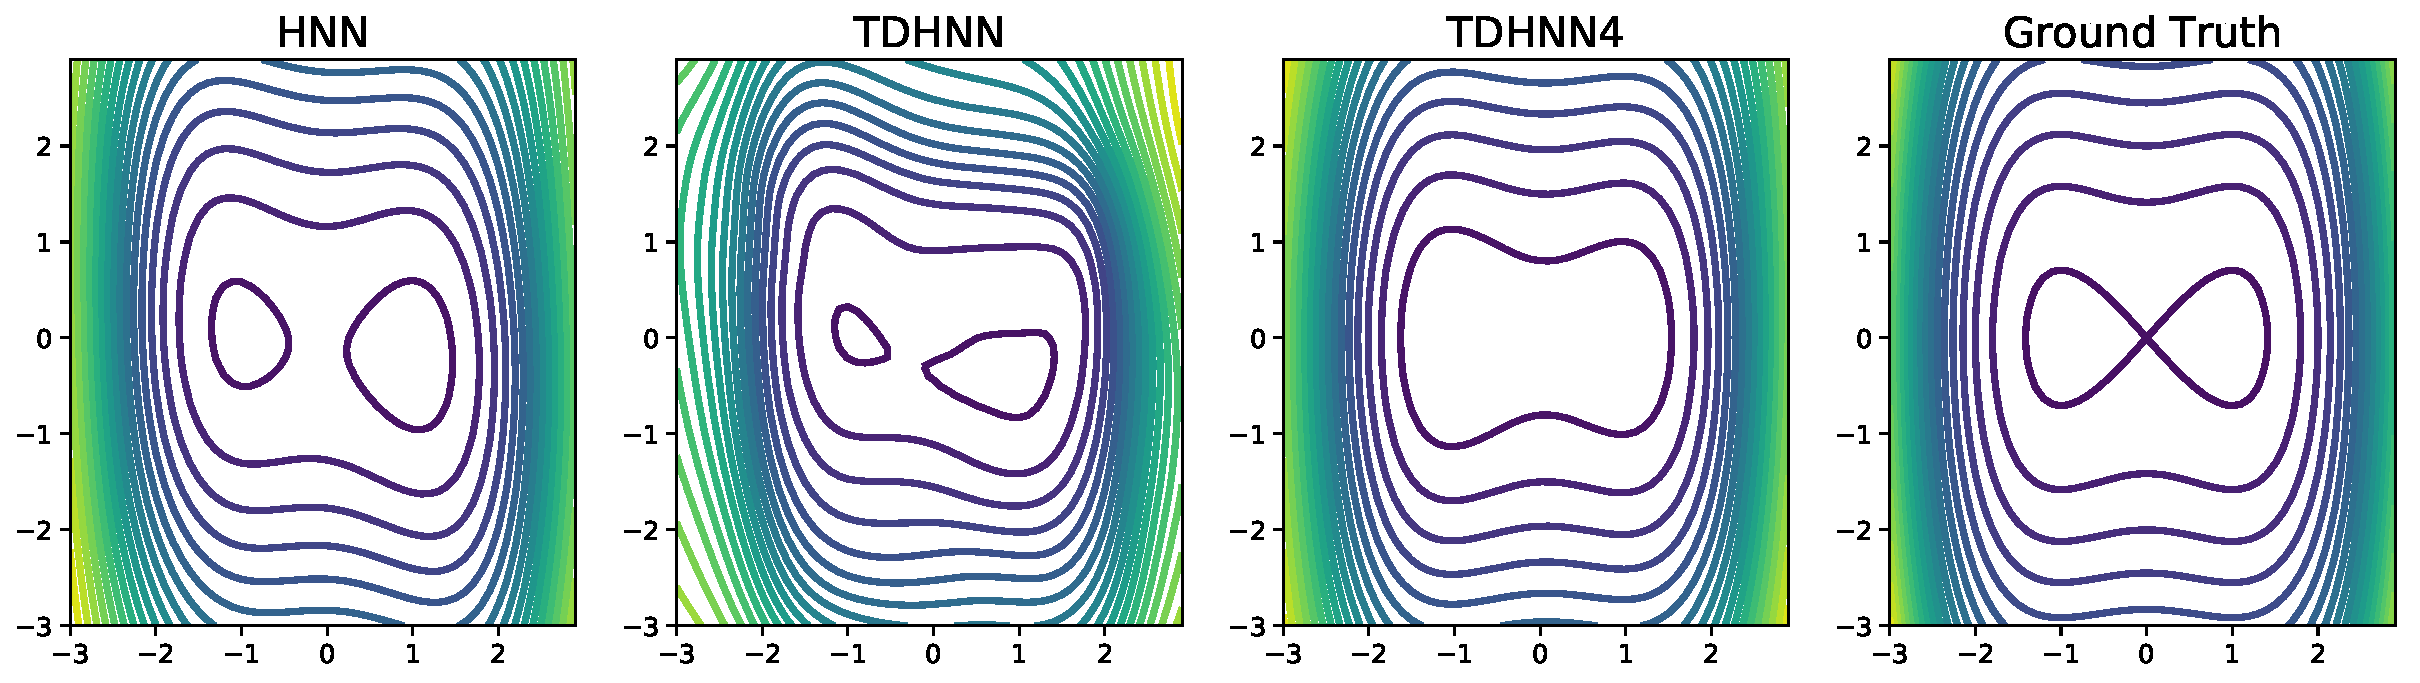
\includegraphics[width=0.9\textwidth]{figures/figures/duffing/1/duffing_hamiltonian_0.pdf}
\caption{Learnt $\mathcal{H}_{reg}$ components across methods in the non-chaotic Duffing setting. HNN and TDHNN learn distorted Hamiltonians that strongly depend on the input time-variable.}
\label{duffing_ham}
\end{figure*}


\subsubsection{Chaotic Regime}

In the chaotic regime we use the following parameters:
$\alpha =1,\beta=1,\delta=0.1,\gamma=0.39,\omega=1.4$. 

\textbf{Training:} 20 initial conditions, sampled uniformly in $[-1,1]^2$ each rolled out for one period $T=2\pi/\omega$ where $\Delta t = T/100$. This results in 2000 training points.

\textbf{Test:} We test our system by assessing whether it is visually able to recover the ground truth Poincar\'e section of an initial condition. The Poincar\'e map of a trajectory is measured by plotting the position and momentum values at regular intervals governed by the period of the forcing term. For example, a simple mass-spring system will generate a single point in phase space when measured at regular intervals. To visually asses the performance of our network through a Poincar\'e map, we test the system on a single initial condition not in the training set rolled out to $T_{\max} = 18,000$ with the same $\Delta t$ as training. In order to integrate our system to such a large $T_{\max}$ for this example we work under the assumption that we have explicit knowledge of the period, and as such, we modulo the time variable with the period. This is necessary as the models are not explicitly trained on time steps beyond $2\pi/\omega$. Our results are visually presented in Fig.\ref{fig.chaos1}. The outcome suggests that pHNN can indeed be used to identify chaos even after being trained with only a few data points from a chaotic trajectory. We believe this is a deeply powerful result in helping us identify chaotic trajectories.

\begin{table*}[hbt!]
\label{tab.table1}
\centering
\caption{State and Energy MSE for each method averaged across 25 initial test points}
\resizebox{\textwidth}{!}{%
    \begin{tabular}{|l|c|c|c|c|c|c|c|c|}
    \toprule
          & \multicolumn{2}{c|}{\textbf{Baseline}} & \multicolumn{2}{c|}{\textbf{HNN}} & \multicolumn{2}{c|}{\textbf{TDHNN}} & \multicolumn{2}{c|}{\textbf{pHNN}} \\
\cmidrule{2-9}          & \textbf{State} & \textbf{Energy} & \textbf{State} & \textbf{Energy} & \textbf{State} & \textbf{Energy} & \textbf{State} & \textbf{Energy} \\
\cmidrule{2-9}    \textbf{Mass Spring} & 1.22E-4 $\pm$ 1.06E-4 & 1.56E-5 $\pm$ 1.84 E-5 & \textbf{1.33E-5 $\pm$ 8.05E-6} & \textbf{1.30E-6 $\pm$ 1.31E-6} & 7.84E-5$\pm$1.02E-4 & 9.26E-6 $\pm$ 1.13E-5 & 2.91E-5 $\pm$ 2.57E-5 & 2.33E-6 $\pm$ 2.41E-6 \\
    \textbf{Damped Mass-Spring} & 6.4E-5 $\pm$ 2.904E-5 & 4.68E-7 $\pm$ 7.51E-7 & 2.81E-1$\pm$ 1.37E-1 & 1.81E-1 $\pm$ 1.37E-1 & 3.01E-1$\pm$1.43E-1 & 1.92E-1$\pm$1.42E-1 & \textbf{1.74E-6$\pm$7.26E-7} & \textbf{1.08E-7$\pm$1.73E-7} \\
    \textbf{Forced (I)} & 5.21E-4 $\pm$ 5.74E-4 & 7.77E-4 $\pm$ 5.52E-4 & 2.36E-1 $\pm$ 1.43E-1 & 2.34E-1 $\pm$ 1.70E-1 & 2.91E-1 $\pm$ 3.06E-1 & 7.61E-1 $\pm$ 1.23 & \textbf{1.53E-5 $\pm$ 1.16E-5} & \textbf{9.21E-6 $\pm$ 7.11E-6} \\
    \textbf{Forced (II)} & 3.14E-2 $\pm$ 2.54E-2 & 7.00E-2 $\pm$ 1.14E-1 & 3.11E-2 $\pm$ 2.67E-2 & 2.70E-2 $\pm$ 1.12E-2 & 2.22E-1 $\pm$ 2.82E-1 & 4.68E-1 $\pm$ 1.06 & \textbf{4.51E-4 $\pm$ 4.85E-4} & \textbf{8.91E-5 $\pm$ 1.01E-4} \\
    \textbf{Duffing} & 1.11E-2 $\pm$ 2.43E-2 & 8.93E-4 $\pm$ 8.75E-4 & 2.31 $\pm$ 1.21 & 4.90 $\pm$ 5.30 & 2.91 $\pm$ 3.01 & 2.43E1 $\pm$ 5.11E1 & \textbf{3.50E-4 $\pm$3.54E-4} & \textbf{5.32E-5 $\pm$ 5.38E-5} \\
    \textbf{Relativistic Duffing} & 5.85E-2 $\pm$ 7.05E-2 & 3.61E-2 $\pm$ 4.76E-2 & 1.39 $\pm$ 1.66 & 2.37E-1 $\pm$ 1.55E-1 & 5.9E-1 $\pm$ 1.44 & 4.39E-2 $\pm$ 5.34E-2 & \textbf{4.96E-3 $\pm$ 8.61E-3} & \textbf{1.28E-3$\pm$1.45E-3} \\
    \bottomrule
\end{tabular}
}%
\end{table*}

\subsection{Relativistic System}
We also go beyond the classical approach and investigate the Duffing equation in a relativistic framework. The Hamiltonian under consideration is:
\begin{equation}
\mathcal{H} =  c\sqrt{p^2 +m_0^2c^2} + \frac{\alpha}{2}q^2 +\frac{\beta}{4}q^4 - q\gamma\sin(\omega t),
\end{equation}
where $c$, the speed of light is typically set to 1. For simplicity, we also set the rest mass $m_0=1$ though our framework naturally accounts for other values.

\textbf{Training:} We train on 25 initial conditions, sampled in $[0,2]^2$ uniformly. $T_{\max} = 20.01$ and $\Delta t = 0.01$. We set parameters such that $\alpha =1, \beta =1,\delta =0,\gamma = 0.2,\omega = 1.2$.

\textbf{Test:} Using the same parameters as training, we rollout 25 unseen initial conditions and compute their state/energy MSE.

\section{Discussion}

We have shown that pHNN can not only outperform other approaches in learning complex physical systems (see Table.1) but can also help us recover the underlying force and damping terms of non-autonomous systems. One challenge in achieving this result is fine-tuning the $\lambda_F$ and $\lambda_N$ regularisation coefficients for the force and damping. In the Duffing setting where we have both terms, it is possible to learn a shifted force i.e. $F = F_0 + \epsilon$. The reason this is possible is because the state-vectors $\mathbf{q},\mathbf{p}$ do not provide enough information to simultaneously identify both the Hamiltonian and the force. As such it is possible that our hyper-parameter selection routine will pick coefficients that maintain a force or damping term in settings where they might not exist. However, we do find that in general a reasonable force and damping term are learnt so as to reveal the underlying dynamics.

In many settings we find that the classic Hamiltonian Neural Network approach or its time-dependent variant simply do not perform as well as pHNN or baseline. We believe this is predominantly due to the fact that HNN and TDHNN attempt to enforce Hamilton's equations in settings where they cannot be satisfied by simply learning a single scalar Hamiltonian. In fact, this is perhaps the main reason why baseline does well because it does not enforce any structure.

While it may be argued that the method is constrained to learning and prediction within the training time horizon, we believe our method is still versatile at informing us of periodic forcing (since we can inspect the force over time). This in turn can readily be used to renormalize the time variable at periodic intervals to integrate the system beyond the training time as we show in Fig.\ref{fig.chaos1}.

\section{Conclusion}

We have shown that learning the dynamics of time-dependent non-autonomous systems can be achieved with pHNN, a versatile neural network embedded with a Port-Hamiltonian designed to recover the underlying Hamiltonian, damping and forcing terms. We show that such an approach, unique in its own right, outperforms naive extensions of existing methods. We believe this work forms a strong basis for further advances in learning complex systems including, but not limited to, chemical bond forces and controlled dynamics without explicit knowledge of the force or damping. Future work in this direction is likely to explore how such a port Hamiltonian approach can be used for many-body systems with more complex forcing.

\pagebreak

\bibliography{references.bib}

\end{document}